\chapter{Metodologia}
\label{cap:metodologia}

\section{Caracteriza\c{c}\~ao}
\label{sec:caracterizacao}

Foram investigados m\'etodos de vis\~ao computacional para identificar, delimitar, localizar e organizar espacialmente parcelas experimentais de forrageiras em imagens orbitais e de drone. Na continuidade proposta nesta qualifica\c{c}\~ao, a composi\c{c}\~ao do conjunto de treinamento passa a ser tratada como vari\'avel experimental, para avaliar se uma sele\c{c}\~ao de imagens orientada por um crit\'erio quantitativo de instabilidade das predi\c{c}\~oes altera a capacidade de generaliza\c{c}\~ao do detector. A identifica\c{c}\~ao das parcelas \'e tratada como etapa de suporte \`a an\'alise dos experimentos e \`a fenotipagem. O sistema n\~ao mede caracter\'isticas como biomassa, altura ou produtividade; seu objetivo \'e localizar e delimitar as parcelas nas imagens e associ\'a-las \`as unidades experimentais previstas no ensaio.

O desenvolvimento foi incremental. Em momentos distintos, foram investigadas a segmenta\c{c}\~ao de inst\^ancias, a detec\c{c}\~ao por caixas delimitadoras horizontais e orientadas, a detec\c{c}\~ao em cascata, a localiza\c{c}\~ao por mapas de confian\c{c}a e um classificador auxiliar de dificuldade das imagens. Tamb\'em foi implementado um procedimento que transfere identificadores de parcelas entre imagens de um mesmo campo a partir de uma refer\^encia numerada. Esses componentes n\~ao formam um fluxo \'unico: alguns foram implementados e avaliados, outros foram conduzidos como linhas independentes, e parte das propostas n\~ao chegou a ser implementada ainda.

\section{Vis\~ao geral}
\label{sec:visao-geral-metodologia}

O processo metodol\'ogico parte da imagem da \'area experimental e chega \`as informa\c{c}\~oes espaciais das parcelas (Figura~\ref{fig:processo-metodologico}). Compreende a obten\c{c}\~ao e a organiza\c{c}\~ao das imagens, a anota\c{c}\~ao das parcelas, a organiza\c{c}\~ao dos conjuntos de dados, o treinamento dos modelos, a extra\c{c}\~ao das posi\c{c}\~oes das parcelas a partir das sa\'idas, a avalia\c{c}\~ao das predi\c{c}\~oes em rela\c{c}\~ao \`as anota\c{c}\~oes de refer\^encia e a associa\c{c}\~ao das detec\c{c}\~oes \`a organiza\c{c}\~ao espacial do experimento. A avalia\c{c}\~ao de estrat\'egias de composi\c{c}\~ao do conjunto de treinamento \'e a etapa prevista para a continuidade do trabalho.

\begin{figure}[htb]
  \centering
  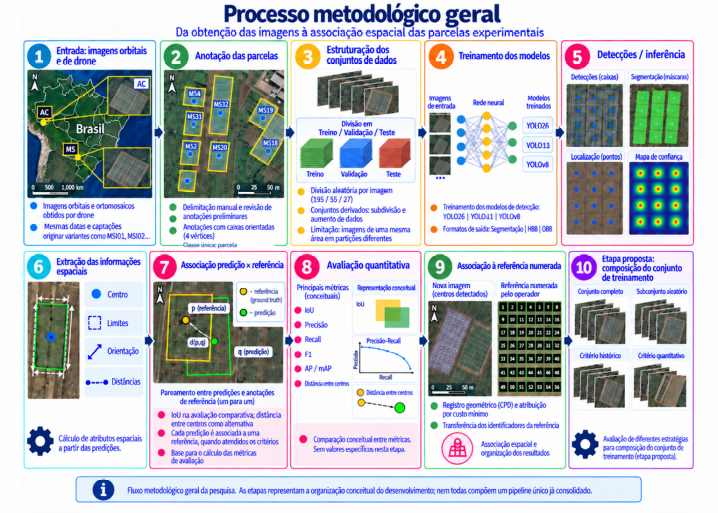
\includegraphics[width=0.95\textwidth]{figuras/figura13.png}
  \caption{Processo metodol\'ogico geral da pesquisa.}
  \label{fig:processo-metodologico}
  \fonte{Elaborado pelo autor (2026).}
\end{figure}

A sequ\^encia descreve a organiza\c{c}\~ao da pesquisa, e n\~ao um fluxo integrado. A detec\c{c}\~ao e a extra\c{c}\~ao das posi\c{c}\~oes foram implementadas, assim como a rotina que associa as detec\c{c}\~oes de novas imagens a uma refer\^encia previamente numerada. Essa rotina usa registro geom\'etrico e atribui\c{c}\~ao entre objetos; ela n\~ao l\^e um arquivo de croqui e ainda n\~ao identifica posi\c{c}\~oes experimentais que ficaram sem detec\c{c}\~ao.

\section{Origem e organiza\c{c}\~ao das imagens}
\label{sec:origem-organizacao-imagens}

As imagens orbitais foram obtidas no \textit{Google Earth}, em sua maioria por captura de tela, e re\'unem diferentes \'areas experimentais e, em alguns casos, a mesma \'area em datas distintas do hist\'orico de imagens. Os ortomosaicos foram gerados a partir de imagens obtidas por drone em campos experimentais da Embrapa Gado de Corte e incorporados ao conjunto de dados.

Quando uma \'area aparece em mais de uma data, mant\'em-se o identificador do campo e acrescenta-se um \'indice \`a varia\c{c}\~ao temporal (por exemplo, \textit{MS10-1} e \textit{MS10-2}), de modo que as imagens permane\c{c}am associadas ao mesmo campo.

Parte dos arquivos traz no nome a data e a hora da captura de tela, que n\~ao correspondem \`a data de aquisi\c{c}\~ao da imagem. A Figura~\ref{fig:organizacao-anual} exemplifica a organiza\c{c}\~ao anual das imagens hist\'oricas de uma mesma \'area.

\begin{figure}[htb]
  \centering
  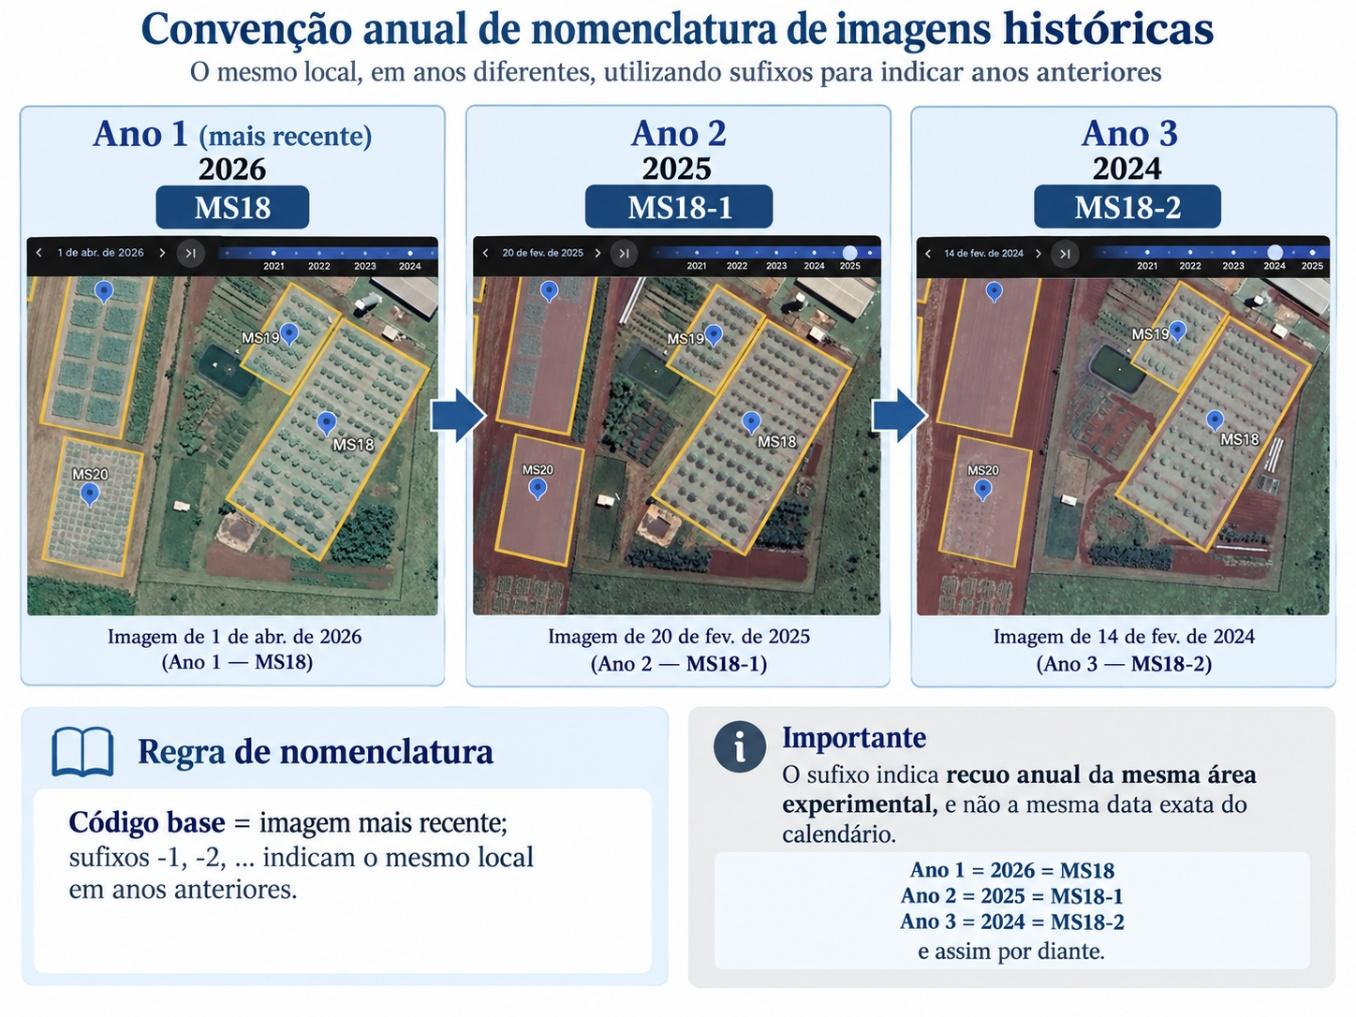
\includegraphics[width=0.95\textwidth]{figuras/figura14.jpg}
  \caption{Organiza\c{c}\~ao anual das imagens hist\'oricas de uma mesma \'area experimental.}
  \label{fig:organizacao-anual}
  \fonte{Elaborado pelo autor (2026).}
\end{figure}

\section{Evolu\c{c}\~ao e organiza\c{c}\~ao dos conjuntos de dados}
\label{sec:evolucao-conjuntos-dados}

O acervo anotado foi constru\'ido em quatro coletas. A primeira reuniu uma imagem orbital por campo experimental, de uma mesma data, e resultou em 35 imagens e 3.444 parcelas. A segunda cobriu 16 campos em diferentes datas do hist\'orico do \textit{Google Earth}, com 54 imagens e 8.179 parcelas anotadas por pol\'igonos. A terceira acrescentou ortomosaicos obtidos por drone, e a quarta, em andamento, abrange 1.045 campos experimentais marcados no \textit{Google Earth}. O conjunto usado nos experimentos mais recentes tem 277 imagens, 156 orbitais e 121 de drone, e 51.245 parcelas anotadas por quatro v\'ertices, isto \'e, como caixas orientadas. Nenhuma imagem da primeira coleta faz parte desse conjunto, enquanto todas as imagens da organiza\c{c}\~ao usada na localiza\c{c}\~ao por pontos est\~ao nele.

Nas primeiras coletas, as anota\c{c}\~oes foram feitas manualmente na plataforma Roboflow. Na terceira coleta, e tamb\'em na quarta, em andamento, adota-se um procedimento \textit{human-in-the-loop}: um modelo j\'a treinado gera anota\c{c}\~oes preliminares, que s\~ao conferidas e, quando necess\'ario, corrigidas manualmente. Trata-se de um procedimento de trabalho, e n\~ao de um m\'odulo do sistema.

As parcelas foram anotadas em uma \'unica classe, parcela, sem categorias para posi\c{c}\~oes vazias ou parcelas mortas. O conjunto de 277 imagens foi exportado da plataforma de anota\c{c}\~ao em abril de 2026, sem aumento de dados, e dividido aleatoriamente por imagem em 195 imagens de treinamento, 55 de valida\c{c}\~ao e 27 de teste. A parti\c{c}\~ao de teste, usada na avalia\c{c}\~ao comparativa dos detectores (Se\c{c}\~ao~\ref{sec:avaliacao-comparativa}), tem 7.852 parcelas; 12 de suas imagens s\~ao de drone e re\'unem 6.667 dessas parcelas.

Dois conjuntos derivados foram gerados a partir desse conjunto pelos procedimentos de prepara\c{c}\~ao descritos adiante. A subdivis\~ao das imagens densas resultou em 384 imagens (258 de treinamento, 80 de valida\c{c}\~ao e 46 de teste), com cada recorte mantido na parti\c{c}\~ao da imagem de origem. O segundo conjunto acrescenta vers\~oes transformadas ao treinamento, que passa a ter 3.406 imagens, e mant\'em a valida\c{c}\~ao e o teste do conjunto subdividido (80 e 46 imagens). O arquivo descritor desse segundo conjunto, contudo, aponta para os diret\'orios do conjunto subdividido; por isso, o treinamento do \textit{YOLO26m} realizado em agosto de 2026, que registra esse descritor, utilizou 258 imagens de treinamento sem as vers\~oes transformadas.

Os 1.045 campos da quarta coleta foram marcados no \textit{Google Earth}, e suas imagens orbitais s\~ao obtidas a partir dessas coordenadas com a biblioteca \textit{leafmap}, uma por campo. Com os novos ortomosaicos obtidos por drone, o acervo deve ultrapassar 1.200 imagens de campo. Essas imagens ainda n\~ao fazem parte dos conjuntos anotados usados nos experimentos apresentados neste trabalho. A Tabela~\ref{tab:conjuntos-dados} re\'une a composi\c{c}\~ao e o uso de cada conjunto.

\begin{table}[htb]
\centering
\caption{Conjuntos de dados do projeto}
\label{tab:conjuntos-dados}
\small
\begin{tabular}{p{3.3cm}p{5.7cm}p{5.7cm}}
\hline
\textbf{Conjunto} & \textbf{Composi\c{c}\~ao} & \textbf{Uso no projeto} \\
\hline
Primeira coleta & 35 imagens e 3.444 parcelas; 26 de treinamento, 6 de valida\c{c}\~ao e 3 de teste & Constru\c{c}\~ao inicial do acervo \\
Segunda coleta & 54 imagens e 8.179 parcelas; 39 de treinamento, 10 de valida\c{c}\~ao e 5 de teste; anota\c{c}\~oes poligonais & Amplia\c{c}\~ao do acervo anotado \\
Organiza\c{c}\~ao para localiza\c{c}\~ao por pontos & 54 imagens; 46 de treinamento, 5 de valida\c{c}\~ao e 3 de teste; anota\c{c}\~oes pontuais & Linha de localiza\c{c}\~ao por mapas de confian\c{c}a \\
Conjunto de 277 imagens (dataset6-OBB) & 277 imagens (156 orbitais e 121 de drone) e 51.245 parcelas; 195 de treinamento, 55 de valida\c{c}\~ao e 27 de teste; caixas orientadas & Parti\c{c}\~ao de teste (27 imagens, 7.852 parcelas) usada na avalia\c{c}\~ao comparativa; origem dos conjuntos derivados \\
Conjunto subdividido (dataset\_imgs\_split) & 384 imagens; 258 de treinamento, 80 de valida\c{c}\~ao e 46 de teste & Treinamento do YOLO26m (agosto de 2026) \\
Conjunto com aumento pr\'evio (dataset\_imgs\_aug) & 3.532 imagens; 3.406 de treinamento, 80 de valida\c{c}\~ao e 46 de teste & Caixas orientadas de maio e agosto de 2026 \\
Coleta por coordenadas & 1.045 campos, uma imagem orbital por campo; com os novos ortomosaicos de drone, mais de 1.200 imagens & Ainda n\~ao utilizada nos experimentos apresentados \\
\hline
\end{tabular}
\end{table}

\section{Depend\^encia entre imagens nas parti\c{c}\~oes}
\label{sec:dependencia-imagens-particoes}

No conjunto de 277 imagens, a divis\~ao aleat\'oria por imagem colocou em parti\c{c}\~oes diferentes imagens de uma mesma \'area. As imagens do quadrante Q5, obtidas em seis datas, est\~ao nas tr\^es parti\c{c}\~oes: quatro no treinamento, uma na valida\c{c}\~ao e uma no teste. As imagens identificadas como quadrante 12 tamb\'em aparecem nas tr\^es parti\c{c}\~oes, e as dos quadrantes Q4 e 15, no treinamento e na valida\c{c}\~ao. A organiza\c{c}\~ao de 54 imagens usada na localiza\c{c}\~ao por pontos apresenta a mesma situa\c{c}\~ao.

H\'a tamb\'em recortes de uma mesma captura de tela em parti\c{c}\~oes diferentes. Em duas capturas, recortes distintos foram para o treinamento e para o teste; em uma delas, o recorte do treinamento est\'a quase inteiramente contido no recorte do teste. Em uma terceira captura, os recortes ficaram no treinamento e na valida\c{c}\~ao. Al\'em disso, v\'arias capturas foram feitas em sequ\^encia, com poucos segundos de intervalo, e distribu\'idas entre parti\c{c}\~oes, de modo que parte delas pode cobrir \'areas iguais ou adjacentes.

Com essa organiza\c{c}\~ao, parte das imagens de valida\c{c}\~ao e de teste est\'a espacialmente relacionada a imagens de treinamento. Isso n\~ao implica que o modelo tenha memorizado os campos nem que uma m\'etrica espec\'ifica esteja incorreta, mas reduz a independ\^encia entre treinamento e avalia\c{c}\~ao e limita a leitura das m\'etricas como estimativa de generaliza\c{c}\~ao para \'areas n\~ao vistas \citep{kattenborn2022}. Os resultados da avalia\c{c}\~ao comparativa foram obtidos com essa parti\c{c}\~ao e s\~ao interpretados com essa restri\c{c}\~ao. Nenhuma nova divis\~ao foi criada para substitu\'i-la retrospectivamente.

A prepara\c{c}\~ao dos dados compreende convers\~ao de formato, redimensionamento, subdivis\~ao das imagens e aumento pr\'evio de dados, executados por scripts independentes do fluxo principal, al\'em das transforma\c{c}\~oes aplicadas pela biblioteca durante o treinamento. Um utilit\'ario converte arquivos \textit{TIFF} em imagens \textit{JPEG}, em RGB e com qualidade 90. A convers\~ao aplica compress\~ao com perdas e n\~ao transfere as informa\c{c}\~oes de georreferenciamento dos arquivos \textit{GeoTIFF} obtidos na coleta por coordenadas.

Imagens com largura inferior a 1.024 \textit{pixels} s\~ao ampliadas por interpola\c{c}\~ao bic\'ubica, com preserva\c{c}\~ao da propor\c{c}\~ao; as demais n\~ao s\~ao alteradas. A amplia\c{c}\~ao aumenta as dimens\~oes das parcelas em pixels, mas n\~ao recupera detalhe ausente da imagem original. A subdivis\~ao foi adotada para limitar o n\'umero de objetos por amostra nas imagens muito densas, de modo que cada recorte tenha, em geral, at\'e cerca de 500 parcelas.

Ap\'os o redimensionamento, imagens com 101 a 500 objetos s\~ao gravadas inteiras. As demais s\~ao percorridas por uma grade de recortes de 1.024 \textit{pixels}, com recortes menores nas bordas. Em cada recorte, contam-se os objetos cujo centro est\'a dentro de seus limites; se a contagem passar de 500 e o recorte tiver mais de 384 \textit{pixels} nas duas dimens\~oes, ele \'e dividido em quatro quadrantes, e o procedimento se repete em cada um. Caso contr\'ario, o recorte \'e gravado.

Com esse crit\'erio, um recorte que j\'a n\~ao pode ser dividido \'e gravado mesmo com mais de 500 objetos, e recortes com menos de 101 objetos tamb\'em s\~ao gravados. A faixa de 101 a 500 objetos \'e o intervalo visado, e n\~ao uma propriedade de todos os recortes.

\subsection{Tratamento das anota\c{c}\~oes nos recortes}
\label{sec:tratamento-anotacoes-recortes}

As coordenadas das anota\c{c}\~oes, originalmente normalizadas em rela\c{c}\~ao \`a imagem inteira, s\~ao convertidas para \textit{pixels}, ajustadas ao sistema de coordenadas do recorte e re-normalizadas em rela\c{c}\~ao \`as suas dimens\~oes. Cada anota\c{c}\~ao \'e atribu\'ida a um recorte pela posi\c{c}\~ao de seu centro, calculado como a m\'edia dos v\'ertices. Uma parcela que intersecta o recorte, mas cujo centro est\'a fora dele, n\~ao \'e inclu\'ida.

Anota\c{c}\~oes poligonais s\~ao recortadas nas bordas e descartadas se ficarem com menos de tr\^es v\'ertices ou com \'area inferior a 4 \textit{pixels} quadrados. Caixas s\~ao reduzidas \`a interse\c{c}\~ao com o recorte e descartadas quando essa interse\c{c}\~ao \'e degenerada ou quando o centro da caixa resultante fica fora do recorte. O procedimento evita anota\c{c}\~oes degeneradas nas bordas, mas uma parcela truncada pode n\~ao representar adequadamente a parcela original.

Um segundo script gera vers\~oes transformadas das imagens e das anota\c{c}\~oes, com rota\c{c}\~ao, cisalhamento, varia\c{c}\~ao de escala, distor\c{c}\~ao de perspectiva e varia\c{c}\~ao de contraste. Na configura\c{c}\~ao do script, cada imagem gera doze variantes, com \^angulos de 0\textdegree{} a 330\textdegree{} em passos de 30\textdegree{}, e a imagem original \'e copiada para o conjunto derivado. Os demais par\^ametros s\~ao sorteados nos intervalos de -15\textdegree{} a 15\textdegree{} (cisalhamento), 0,5 a 1,5 (escala), at\'e 0,05 (perspectiva) e 0,5 a 1,75 (contraste). A supress\~ao de regi\~oes da imagem est\'a implementada, mas desativada.

O sorteio usa um gerador pseudoaleat\'orio com semente 42, o que n\~ao garante, sozinho, a reprodu\c{c}\~ao exata das imagens transformadas, que depende tamb\'em da biblioteca e da ordem de processamento. Para transformar as anota\c{c}\~oes, cada parcela \'e rasterizada em uma m\'ascara pr\'opria, e todas as m\'ascaras recebem a mesma transforma\c{c}\~ao geom\'etrica aplicada \`a imagem. Os contornos externos s\~ao ent\~ao extra\'idos m\'ascara a m\'ascara, o que evita que parcelas vizinhas que passem a se tocar ap\'os a transforma\c{c}\~ao sejam reconstru\'idas como um \'unico objeto.

Os r\'otulos resultantes s\~ao pol\'igonos com n\'umero vari\'avel de v\'ertices, e o procedimento n\~ao garante a conserva\c{c}\~ao de todas as inst\^ancias originais. As imagens geradas derivam das mesmas imagens de origem e n\~ao constituem observa\c{c}\~oes independentes.

\subsection{Transforma\c{c}\~oes durante o treinamento}
\label{sec:transformacoes-treinamento}

A configura\c{c}\~ao de treinamento tamb\'em define transforma\c{c}\~oes aplicadas pela biblioteca no carregamento das amostras, como composi\c{c}\~ao em mosaico, mistura de imagens, altera\c{c}\~oes geom\'etricas e ajustes de cor, segundo as probabilidades e condi\c{c}\~oes da pr\'opria biblioteca. Os valores da configura\c{c}\~ao atual n\~ao estabelecem os que foram usados nos treinamentos anteriores. O conjunto com aumento pr\'evio cont\'em vers\~oes transformadas apenas no treinamento, enquanto a vers\~ao atual do script processa somente os subconjuntos de valida\c{c}\~ao.

O script de prepara\c{c}\~ao processa separadamente treinamento, valida\c{c}\~ao e teste e grava as sa\'idas nas parti\c{c}\~oes correspondentes, de modo que cada recorte permanece na parti\c{c}\~ao de sua imagem de origem. Isso n\~ao elimina a depend\^encia descrita em ``Depend\^encia entre imagens nas parti\c{c}\~oes''. N\~ao h\'a resultados de compara\c{c}\~oes controladas que isolem o efeito do redimensionamento, da subdivis\~ao ou do aumento de dados sobre o desempenho.

\section{Abordagens de vis\~ao computacional investigadas}
\label{sec:abordagens-investigadas}

As formas investigadas para identificar e localizar as parcelas diferem pela representa\c{c}\~ao de sa\'ida. A segmenta\c{c}\~ao de inst\^ancias delimita cada parcela por m\'ascara ou contorno \citep{he2017}; a detec\c{c}\~ao por caixas horizontais representa cada parcela por um ret\^angulo alinhado aos eixos da imagem, como na formula\c{c}\~ao original da fam\'ilia \textit{YOLO} \citep{redmon2016}; a detec\c{c}\~ao por caixas orientadas acrescenta a esse ret\^angulo um \^angulo \citep{ding2019}; e a localiza\c{c}\~ao por mapas de confian\c{c}a produz uma resposta cont\'inua cujos m\'aximos indicam as posi\c{c}\~oes das parcelas \citep{arruda2022}. Tamb\'em foram treinados um detector em cascata e um classificador auxiliar, este sem fun\c{c}\~ao de localiza\c{c}\~ao.

A representa\c{c}\~ao de sa\'ida n\~ao se confunde com a gera\c{c}\~ao da fam\'ilia \textit{YOLO} nem com o tamanho do modelo: diferentes gera\c{c}\~oes foram usadas, e uma mesma gera\c{c}\~ao foi treinada com representa\c{c}\~oes diferentes. As linhas investigadas t\^em n\'iveis distintos de maturidade e n\~ao foram conduzidas sob um mesmo protocolo. Os checkpoints \textit{YOLO} de segmenta\c{c}\~ao, caixas horizontais e caixas orientadas foram avaliados sobre um conjunto de teste comum (Se\c{c}\~ao~\ref{sec:avaliacao-comparativa}). A localiza\c{c}\~ao por mapas de confian\c{c}a e a detec\c{c}\~ao em cascata n\~ao fazem parte dessa avalia\c{c}\~ao.

A segmenta\c{c}\~ao de inst\^ancias foi uma das primeiras linhas investigadas. O modelo recebe a imagem e produz uma m\'ascara para cada parcela identificada, com treinamento supervisionado pelas anota\c{c}\~oes poligonais. Foram usadas as gera\c{c}\~oes \textit{YOLOv8, YOLO11 e YOLO26} \citep{jocher2026}, por meio da biblioteca \textit{Ultralytics} \citep{jocher2023}. Esses modelos foram treinados em momentos distintos, com diferen\c{c}as de tamanho de entrada, tamanho de lote, n\'umero de \'epocas e demais configura\c{c}\~oes, de modo que seus resultados n\~ao constituem uma compara\c{c}\~ao controlada entre gera\c{c}\~oes.

Na detec\c{c}\~ao por caixas horizontais, cada parcela \'e representada por uma caixa alinhada aos eixos da imagem. O interesse est\'a na presen\c{c}a e na posi\c{c}\~ao da parcela, sem delimitar o contorno da vegeta\c{c}\~ao, e o centro da caixa \'e obtido diretamente, o que simplifica a localiza\c{c}\~ao e a ordena\c{c}\~ao espacial.

A detec\c{c}\~ao por caixas orientadas representa cada parcela por um ret\^angulo acrescido de um par\^ametro de orienta\c{c}\~ao, de modo que a predi\c{c}\~ao \'e descrita por posi\c{c}\~ao, dimens\~oes e \^angulo. Essa formula\c{c}\~ao permite descrever objetos cuja dire\c{c}\~ao predominante n\~ao coincide com os eixos horizontal e vertical da imagem, condi\c{c}\~ao frequente em imagens a\'ereas \citep{ding2019,ding2022}. Em um contexto especificamente agr\'icola, \citet{zhang2025} avaliam uma rede de segmenta\c{c}\~ao orientada voltada \`a extra\c{c}\~ao de parcelas de melhoramento rotacionadas em imagens RGB de VANT, tratando a orienta\c{c}\~ao como parte expl\'icita da representa\c{c}\~ao.

A orienta\c{c}\~ao passou a ser tratada explicitamente para lidar com imagens nas quais as parcelas aparecem rotacionadas em rela\c{c}\~ao aos eixos. Na primeira coleta, a rota\c{c}\~ao era corrigida antes da captura das imagens, e as parcelas eram anotadas com caixas sem inclina\c{c}\~ao. Duas alternativas foram consideradas: ampliar o conjunto com rota\c{c}\~oes das mesmas imagens, com risco de sobreajuste, ou adotar uma representa\c{c}\~ao que aprendesse a orienta\c{c}\~ao, o que acrescenta um par\^ametro angular \`a caixa. A segunda levou aos modelos de caixas orientadas, e o aumento pr\'evio com rota\c{c}\~oes tamb\'em foi implementado. A delimita\c{c}\~ao exata do contorno, obtida pela segmenta\c{c}\~ao, foi considerada desnecess\'aria para a fenotipagem realizada na Embrapa Gado de Corte, o que justificou o uso de caixas nessa aplica\c{c}\~ao. Os checkpoints de caixas orientadas s\~ao os mais recentes do projeto, e um deles, \textbf{260525\_2231}, \'e o modelo indicado na configura\c{c}\~ao do sistema para infer\^encia.

Checkpoints das tr\^es representa\c{c}\~oes foram avaliados sobre o mesmo conjunto de teste, mas essa avalia\c{c}\~ao n\~ao \'e uma abla\c{c}\~ao da representa\c{c}\~ao geom\'etrica: os treinamentos ocorreram em etapas diferentes, com configura\c{c}\~oes e conjuntos de treinamento distintos. Diferen\c{c}as de desempenho n\~ao podem, portanto, ser atribu\'idas apenas \`a orienta\c{c}\~ao das caixas.

\section{Localiza\c{c}\~ao por mapas de confian\c{c}a}
\label{sec:localizacao-mapas-confianca}

Uma linha metodol\'ogica distinta, motivada por \citet{arruda2022} e fundamentada na Se\c{c}\~ao~\ref{sec:multistagerefinementnet}, representa as parcelas por mapas de confian\c{c}a em vez de caixas ou m\'ascaras. A sa\'ida da rede \'e um mapa cont\'inuo, e n\~ao uma lista de coordenadas: as posi\c{c}\~oes s\~ao obtidas em p\'os-processamento, pela identifica\c{c}\~ao de m\'aximos locais, e o resultado \'e um conjunto de pontos, sem delimita\c{c}\~ao da extens\~ao de cada parcela. A implementa\c{c}\~ao do projeto, em \textit{TensorFlow} e \textit{Keras}, \'e descrita na subse\c{c}\~ao~\ref{sec:implementacao-mapas-confianca}.

Tamb\'em foi treinado um detector Cascade R-CNN, arquitetura que encadeia est\'agios de detec\c{c}\~ao com limiares de correspond\^encia progressivamente mais estritos \citep{cai2018}, implementado com a biblioteca \textit{MMDetection} e \textit{backbone ResNet-50} \citep{he2016} com FPN \citep{lin2017}. Houve duas execu\c{c}\~oes de 12 \'epocas, com valida\c{c}\~ao ao fim de cada \'epoca, que leram diret\'orios de dados diferentes, cuja equival\^encia n\~ao foi verificada. A linha foi descontinuada antes de uma avalia\c{c}\~ao no conjunto de teste; seus resultados s\~ao apresentados na Se\c{c}\~ao~\ref{sec:linhas-paralelas}.

O classificador auxiliar n\~ao localiza parcelas: classifica cada imagem conforme a dificuldade que ela representa para o detector, a partir de r\'otulos avaliados, sua constru\c{c}\~ao, treinamento e limita\c{c}\~oes s\~ao descritos na subse\c{c}\~ao~\ref{sec:classificador-auxiliar-efficientnet}, ``Classificador auxiliar de dificuldade baseado em EfficientNet-B0''.

\section{Propostas estruturais investigadas para a associa\c{c}\~ao ao croqui}
\label{sec:propostas-estruturais}

Al\'em das abordagens visuais, duas propostas estruturais, \textit{Grid Completion} e \textit{Loss de Matriz}, foram formuladas para relacionar as detec\c{c}\~oes \`a organiza\c{c}\~ao espacial esperada do experimento; ambas s\~ao descritas na subse\c{c}\~ao~\ref{sec:propostas-anteriores-organizacao}, ``Propostas anteriores relacionadas \`a organiza\c{c}\~ao espacial''. A Tabela~\ref{tab:abordagens-papel} re\'une o papel e o estado documentado de cada componente investigado.

\begin{table}[htb]
\centering
\caption{Abordagens visuais, classifica\c{c}\~ao auxiliar e propostas estruturais: papel e estado documentado}
\label{tab:abordagens-papel}
\small
\begin{tabular}{p{4cm}p{4.3cm}p{6.4cm}}
\hline
\textbf{Abordagem ou componente} & \textbf{Representa\c{c}\~ao de sa\'ida} & \textbf{Fun\c{c}\~ao no projeto} \\
\hline
Segmenta\c{c}\~ao de inst\^ancias (YOLOv8, YOLO11, YOLO26) & M\'ascara ou contorno por parcela & Linha inicial de identifica\c{c}\~ao \\
Detec\c{c}\~ao por caixas horizontais (YOLO26) & Ret\^angulo alinhado aos eixos & Representa\c{c}\~ao intermedi\'aria; base geom\'etrica para extra\c{c}\~ao de centros \\
Detec\c{c}\~ao por caixas orientadas (YOLO26) & Ret\^angulo com par\^ametro de orienta\c{c}\~ao & Representa\c{c}\~ao do modelo indicado para infer\^encia \\
Localiza\c{c}\~ao por mapas de confian\c{c}a & Mapa cont\'inuo; posi\c{c}\~oes obtidas por m\'aximos locais no p\'os-processamento & Linha alternativa de localiza\c{c}\~ao e contagem, sem avalia\c{c}\~ao quantitativa \\
Detec\c{c}\~ao em cascata (Cascade R-CNN) & Caixas & Linha descontinuada antes da avalia\c{c}\~ao no conjunto de teste \\
Classificador auxiliar (EfficientNet-B0) & Classe bin\'aria por imagem & Classifica\c{c}\~ao da dificuldade operacional em rela\c{c}\~ao ao detector \\
Grid Completion (proposta estrutural) & Grade te\'orica e c\'elulas sem detec\c{c}\~ao & Implementada em 2025 e removida do c\'odigo em 2026 \\
\hline
\end{tabular}
\end{table}

Os \textit{checkpoints} preservados documentam execu\c{c}\~oes de treinamento feitas ao longo do desenvolvimento, em uma trajet\'oria incremental, e n\~ao um estudo comparativo planejado desde o in\'icio. S\~ao dezesseis \textit{checkpoints} treinados; a Tabela~\ref{tab:experimentos-yolo} apresenta seis deles, um para cada combina\c{c}\~ao principal de gera\c{c}\~ao, tamanho de modelo e representa\c{c}\~ao de sa\'ida. A caracteriza\c{c}\~ao dos treinamentos usa os metadados gravados nos pr\'oprios \textit{checkpoints}: par\^ametros de configura\c{c}\~ao, caminhos dos descritores de dados e hist\'oricos por \'epoca.

O treinamento parte de um \textit{checkpoint} indicado na configura\c{c}\~ao como modelo-base e do descritor do conjunto de dados, e \'e interrompido se algum deles n\~ao estiver dispon\'ivel. Os par\^ametros da configura\c{c}\~ao, o caminho do conjunto de dados e a identifica\c{c}\~ao da execu\c{c}\~ao s\~ao encaminhados \`a biblioteca \textit{Ultralytics}, que conduz o ajuste do modelo. A configura\c{c}\~ao tamb\'em permite retomar uma execu\c{c}\~ao interrompida.

Ao fim de uma execu\c{c}\~ao, o sistema copia o arquivo de melhores pesos com um nome padronizado, formado pelo carimbo de data e hora de modifica\c{c}\~ao do arquivo, pelo nome do modelo-base, por uma identifica\c{c}\~ao de t\'ecnica e pelo mAP@0,5 de valida\c{c}\~ao obtido ao final do treinamento. No treinamento do \textit{YOLO26m} de agosto de 2026, o carimbo \textbf{260810\_2042} coincide com o t\'ermino da execu\c{c}\~ao, e o sufixo \textbf{96\_2} \'e compat\'ivel com o maior \textbf{mAP@0,5} de valida\c{c}\~ao registrado, \textbf{0,96253}, na \'epoca 90. A escolha dos melhores pesos segue o crit\'erio da biblioteca. Os nomes dos \textit{checkpoints} anteriores n\~ao seguem integralmente essa regra e, por isso, n\~ao s\~ao usados para reconstruir sua origem.

\subsection{Procedimentos de valida\c{c}\~ao nos experimentos hist\'oricos}
\label{sec:procedimentos-validacao-historicos}

Parte dos \textit{checkpoints} traz no nome termos de valida\c{c}\~ao cruzada (\textit{leave-one-out} e valida\c{c}\~ao aninhada), e os caminhos de sess\~ao gravados nos metadados confirmam essa organiza\c{c}\~ao. Na sess\~ao \textit{\textbf{nested}\_cv\_20260318\_162914}, os checkpoints \textbf{260318\_2058} e \textbf{260320\_0320} registram as parti\c{c}\~oes externas \textit{outer\_fold\_1} e \textit{outer\_fold\_5}, com limite de 60 \'epocas, e o checkpoint \textbf{260323\_1718}, associado ao diret\'orio \textit{final\_model} da mesma sess\~ao, registra 120 \'epocas.

Os resultados das demais parti\c{c}\~oes e os resultados agregados dessas valida\c{c}\~oes n\~ao est\~ao dispon\'iveis. Um modelo identificado como final n\~ao \'e um resultado agregado de valida\c{c}\~ao cruzada, e o limite de \'epocas registrado para ele n\~ao se aplica \`as parti\c{c}\~oes.

A Tabela~\ref{tab:experimentos-yolo} re\'une os par\^ametros das seis execu\c{c}\~oes, recuperados dos metadados de cada checkpoint. Todas usam o otimizador \textbf{AdamW} \citep{loshchilov2019} e diferem em taxa inicial de aprendizagem, paci\^encia, tamanho de lote e dimens\~ao de entrada; as vers\~oes declaradas da biblioteca e as ra\'izes dos caminhos de arquivos tamb\'em variam entre elas.

\begin{table}[htb]
\centering
\caption{Experimentos com modelos da fam\'ilia YOLO}
\label{tab:experimentos-yolo}
\small
\begin{tabular}{p{1.7cm}p{3.4cm}p{4.2cm}p{1.7cm}p{1cm}p{1.2cm}}
\hline
\textbf{ID} & \textbf{Modelo e tarefa} & \textbf{Evid\^encia do protocolo} & \textbf{\'Epocas config.} & \textbf{Lote} & \textbf{imgsz} \\
\hline
EXP-002 & YOLOv8n, segmenta\c{c}\~ao & \textit{Leave-one-out} (nome e caminho da sess\~ao) & 100 & 8 & 640 \\
EXP-003 & YOLO11n, segmenta\c{c}\~ao & \textit{Leave-one-out} (nome e caminho da sess\~ao) & 100 & 16 & 640 \\
EXP-006 & YOLO26s, segmenta\c{c}\~ao & Valida\c{c}\~ao aninhada, modelo final (caminho da sess\~ao) & 120 & 8 & 1024 \\
EXP-009 & YOLO26s, caixas horizontais & Valida\c{c}\~ao aninhada, modelo final (caminho da sess\~ao) & 120 & 4 & 1024 \\
EXP-013 & YOLO26s, caixas orientadas & Sem valida\c{c}\~ao cruzada & 120 & 8 & 1024 \\
EXP-016 & YOLO26m, caixas orientadas & Sem valida\c{c}\~ao cruzada & 120 & 8 & 1280 \\
\hline
\end{tabular}

\vspace{0.3cm}
\footnotesize \textit{Nota: \'epocas, lote e imgsz (dimens\~ao de entrada, em pixels) foram recuperados dos metadados de configura\c{c}\~ao de cada checkpoint; nas seis execu\c{c}\~oes, o hist\'orico por \'epoca chega ao limite configurado. Os demais par\^ametros, como taxa inicial de aprendizagem, paci\^encia e semente, tamb\'em constam desses metadados. O EXP-016 foi repetido com lote 8 depois que a primeira tentativa, com lote 12, falhou por falta de mem\'oria na GPU na \'epoca 18.}
\end{table}

\subsection{Proveni\^encia dos conjuntos de dados}
\label{sec:proveniencia-conjuntos}

Os metadados registram o caminho do descritor de dados de cada execu\c{c}\~ao. Parte dos \textit{checkpoints} de 2025 e do primeiro semestre de 2026 aponta para descritores de sess\~oes de valida\c{c}\~ao cruzada. Os \textit{checkpoints} \textbf{251004\_2132} e \textbf{251022\_1208} foram treinados com conjuntos ponderados por dificuldade: cada imagem recebeu manualmente um n\'ivel de 1 a 4, e as imagens foram replicadas no treinamento em n\'umero aproximadamente proporcional ao quadrado desse n\'ivel. Os checkpoints de caixas orientadas de maio de 2026 registram os diret\'orios \textit{dataset\_imgs\_aug1} (\textbf{260525\_2231}) e \textit{dataset\_imgs\_aug} (\textbf{260528\_0037} e \textbf{260530\_1336}), e o \textit{YOLO26m} de agosto registra \textit{dataset\_imgs\_aug}.

Os \textit{checkpoints} \textbf{260525\_2231} e \textbf{260530\_1336} ilustram esse limite: o primeiro registra dataset\_imgs\_aug1 e dimens\~ao de entrada de 1.024 pixels; o segundo, \textit{dataset\_imgs\_aug} e 1.280 pixels. As execu\c{c}\~oes diferem na configura\c{c}\~ao e possivelmente nos dados, e por isso a diferen\c{c}a de desempenho descrita nos Resultados n\~ao tem causa identificada.

\subsection{Alcance da compara\c{c}\~ao entre esses experimentos}
\label{sec:alcance-comparacao}

A avalia\c{c}\~ao comparativa aplicou 15 \textit{checkpoints} treinados e o modelo-base sem ajuste ao mesmo teste de 27 imagens, com os mesmos par\^ametros de infer\^encia e de correspond\^encia. Essa condi\c{c}\~ao comum permite comparar os modelos de forma descritiva, mas n\~ao equaliza o treinamento: os \textit{checkpoints} diferem em gera\c{c}\~ao, tamanho, representa\c{c}\~ao de sa\'ida, dimens\~ao de entrada, n\'umero de \'epocas, dados de treinamento e vers\~ao da biblioteca, e nenhuma dessas vari\'aveis foi isolada. \textit{Checkpoints} treinados com uma dimens\~ao de entrada e avaliados com outra podem, al\'em disso, ser afetados por essa diferen\c{c}a. O YOLO26m de agosto de 2026 foi avaliado depois, com dimens\~ao de entrada de 1.280 \textit{pixels} e uma vers\~ao posterior do script de avalia\c{c}\~ao, e seu resultado \'e apresentado \`a parte.

\subsection{Implementa\c{c}\~ao da abordagem baseada em mapas de confian\c{c}a}
\label{sec:implementacao-mapas-confianca}

A implementa\c{c}\~ao dessa abordagem trabalha com uma representa\c{c}\~ao diferente da usada pelos detectores. As posi\c{c}\~oes anotadas s\~ao convertidas em mapas de refer\^encia, amostrados em uma grade de pixels, que servem de alvo ao treinamento; as posi\c{c}\~oes das parcelas s\~ao estimadas depois, por p\'os-processamento.

A entrada dessa linha n\~ao s\~ao r\'otulos poligonais, mas pontos. Um utilit\'ario l\^e as anota\c{c}\~oes quadrilaterais (classe e oito coordenadas normalizadas), calcula a m\'edia dos quatro v\'ertices, converte o resultado para pixels e trunca os valores para inteiros. Cada arquivo passa a conter uma lista de posi\c{c}\~oes, sem classe e sem a extens\~ao da parcela.

No treinamento, a imagem \'e normalizada para o intervalo unit\'ario e redimensionada por interpola\c{c}\~ao bilinear at\'e a dimens\~ao de entrada da rede. As respostas de refer\^encia, por sua vez, s\~ao constru\'idas em uma resolu\c{c}\~ao menor que a da entrada, determinada por um fator de redu\c{c}\~ao. As coordenadas anotadas s\~ao reescaladas para essa resolu\c{c}\~ao por fatores calculados independentemente em cada eixo, a partir da raz\~ao entre as dimens\~oes do mapa e as da imagem original.

Sobre esse mapa, cada objeto produz uma resposta gaussiana bidimensional centrada em sua posi\c{c}\~ao. As respostas de objetos distintos s\~ao combinadas pelo m\'aximo ponto a ponto, e n\~ao por soma; assim, a soma do mapa n\~ao corresponde ao n\'umero de objetos, e objetos muito pr\'oximos podem n\~ao gerar picos distintos. Pontos que saem dos limites do mapa s\~ao descartados.

Cada est\'agio de refinamento tem seu pr\'oprio mapa de refer\^encia, constru\'ido com as mesmas anota\c{c}\~oes e com o desvio padr\~ao da gaussiana decrescendo linearmente entre um valor m\'aximo e um m\'inimo, conforme a motiva\c{c}\~ao do m\'etodo publicado: os est\'agios iniciais aprendem uma localiza\c{c}\~ao aproximada e os finais a refinam \citep{arruda2022}. Os desvios padr\~ao s\~ao ajustados pelo fator de redu\c{c}\~ao de resolu\c{c}\~ao, para que a dispers\~ao acompanhe a escala do mapa.

\subsubsection*{Organiza\c{c}\~ao da rede e op\c{c}\~oes configuradas}

A implementa\c{c}\~ao, denominada no c\'odigo do projeto como \textit{\textbf{MultiStageRefinementNet}}, segue a organiza\c{c}\~ao em tr\^es componentes descrita na Se\c{c}\~ao~\ref{sec:multistagerefinementnet}, com o m\'odulo de agrega\c{c}\~ao em pir\^amide configurado para quatro escalas e cada est\'agio de refinamento recebendo, al\'em da sa\'ida da agrega\c{c}\~ao, o mapa produzido pelo est\'agio anterior.

Os est\'agios n\~ao recebem a mesma entrada. O primeiro est\'agio recebe a sa\'ida do m\'odulo de agrega\c{c}\~ao em pir\^amide. Nos est\'agios seguintes, essa representa\c{c}\~ao \'e concatenada ao mapa de confian\c{c}a produzido pelo est\'agio anterior, permitindo o refinamento sucessivo das respostas. Cada est\'agio produz seu pr\'oprio mapa.

O extrator de caracter\'isticas pode ser a vers\~ao simplificada inspirada na VGG19, sem pr\'e-treino, ou a VGG19 pr\'e-treinada; a configura\c{c}\~ao padr\~ao seleciona a primeira, e um dos treinamentos usou a segunda. A entrada da rede tem 512 $\times$ 512 \textit{pixels}, a redu\c{c}\~ao de resolu\c{c}\~ao padr\~ao \'e de oito vezes, o que resulta em mapas de 64 $\times$ 64 \textit{pixels}, e h\'a quatro est\'agios de refinamento; um dos treinamentos usou redu\c{c}\~ao de quatro vezes.

\subsubsection*{Treinamento definido na implementa\c{c}\~ao}

A fun\c{c}\~ao de perda implementada \'e um erro quadr\'atico ponderado. Cada \textit{pixel} recebe um peso conforme o valor do mapa de refer\^encia naquela posi\c{c}\~ao: \textit{pixels} cujo alvo seja maior ou igual a um limiar recebem um peso maior, e os demais, um peso menor. O erro quadr\'atico ponderado \'e somado e dividido pela soma dos pesos, acrescida de uma pequena constante de estabiliza\c{c}\~ao, de modo que a perda corresponde a uma m\'edia ponderada e n\~ao a uma soma. O prop\'osito declarado no c\'odigo \'e compensar o desbalanceamento entre as regi\~oes de pico e o fundo do mapa, que ocupa a maior parte de sua \'area.

A classe de perda define, por padr\~ao, pesos 8 e 1 para as regi\~oes positivas e de fundo, com limiar de 0,05; o script de treinamento usa pesos 12 e 1 e limiar de 0,03.

Cada est\'agio \'e supervisionado pelo mapa de refer\^encia correspondente; as perdas dos est\'agios s\~ao somadas e divididas pelo n\'umero de imagens do lote. A publica\c{c}\~ao de refer\^encia define, em vez disso, uma soma de erros quadr\'aticos por posi\c{c}\~ao em cada est\'agio, somada entre est\'agios e sem pondera\c{c}\~ao entre regi\~oes \citep{arruda2022}.

A rede produz um mapa de confian\c{c}a por est\'agio. A localiza\c{c}\~ao utiliza o mapa do \'ultimo est\'agio, tanto na rotina de infer\^encia quanto na avalia\c{c}\~ao implementada. A obten\c{c}\~ao das posi\c{c}\~oes ocorre em uma etapa separada de p\'os-processamento, que identifica m\'aximos locais, aplica um limiar de confian\c{c}a e prev\^e supress\~ao opcional por dist\^ancia.

Um \textit{pixel} \'e candidato a m\'aximo local quando seu valor \'e igual ao maior valor de sua vizinhan\c{c}a ortogonal imediata, obtido por dilata\c{c}\~ao com n\'ucleo em cruz; diferentemente da compara\c{c}\~ao estrita da publica\c{c}\~ao de refer\^encia, esse crit\'erio aceita empates. Em seguida, ret\^em-se os candidatos com valor maior ou igual ao limiar de confian\c{c}a, e o script de execu\c{c}\~ao usa um limiar mais permissivo que o padr\~ao da fun\c{c}\~ao. A supress\~ao por dist\^ancia m\'inima, que descartaria candidatos pr\'oximos a outros de maior confian\c{c}a, est\'a fixada em um pixel e, portanto, n\~ao tem efeito.

A detec\c{c}\~ao de picos retorna inicialmente posi\c{c}\~oes na grade do mapa de confian\c{c}a. Em seguida, as coordenadas s\~ao reescaladas separadamente nos eixos horizontal e vertical para as dimens\~oes da imagem original e convertidas para valores inteiros. As posi\c{c}\~oes resultantes representam estimativas de localiza\c{c}\~ao nessa imagem, sem delimita\c{c}\~ao da extens\~ao das parcelas ou atribui\c{c}\~ao de identificadores do croqui. Sua correspond\^encia com parcelas efetivamente presentes dependeria de avalia\c{c}\~ao experimental.

O m\'odulo calcula, para a contagem, erro absoluto m\'edio, raiz do erro quadr\'atico m\'edio e coeficiente de determina\c{c}\~ao. Para a localiza\c{c}\~ao, cada refer\^encia \'e associada \`a primeira predi\c{c}\~ao ainda livre situada a at\'e quatro pixels de dist\^ancia, sem buscar a mais pr\'oxima nem fazer atribui\c{c}\~ao global. Esse crit\'erio difere da correspond\^encia por sobreposi\c{c}\~ao usada na avalia\c{c}\~ao dos detectores, e os valores dos dois protocolos n\~ao s\~ao diretamente compar\'aveis.

Modelos dessa linha foram treinados em diferentes configura\c{c}\~oes, e as m\'etricas de contagem (MAE, RMSE e R\textsuperscript{2}) e de localiza\c{c}\~ao (precis\~ao, recall e F1) foram calculadas no conjunto de valida\c{c}\~ao a cada \'epoca; os valores s\~ao apresentados nos Resultados.

A implementa\c{c}\~ao permanece em m\'odulo separado, sem integra\c{c}\~ao que use um modelo YOLO como extrator de caracter\'isticas.

\section{Classificador auxiliar de dificuldade baseado em \textit{EfficientNet-B0}}
\label{sec:classificador-auxiliar-efficientnet}

O classificador auxiliar estima, a partir da imagem, uma categoria de dificuldade em rela\c{c}\~ao ao detector usado para gerar seus r\'otulos. A sa\'ida n\~ao \'e uma propriedade agron\^omica da \'area, n\~ao identifica parcelas e n\~ao \'e uma medida geral de qualidade da imagem: indica apenas se se espera que o detector tenha desempenho elevado naquela imagem, segundo o crit\'erio descrito a seguir.

Os r\'otulos bin\'arios s\~ao obtidos automaticamente do F1 de cada imagem (coluna f1\_medio) em um arquivo de m\'etricas por imagem gerado em 7 de junho de 2026, com 4.992 registros.

Recebem classe 1 as imagens com F1 maior ou igual a 0,97, e classe 0 as demais. O limiar foi adotado empiricamente, sem deriva\c{c}\~ao estat\'istica, como par\^ametro para construir os r\'otulos; n\~ao \'e uma medida de acur\'acia da rede nem foi usado para selecionar imagens de treinamento do detector. Na data em que esses valores foram gerados, a configura\c{c}\~ao de detec\c{c}\~ao do sistema usava o \textit{checkpoint} 260525\_2231, com confian\c{c}a m\'inima de 0,3, entrada de 1.024 pixels e IoU de correspond\^encia de 0,3.

Os registros s\~ao divididos em 70\% para treinamento, 20\% para valida\c{c}\~ao e 10\% para teste, por duas divis\~oes sucessivas estratificadas pela classe e com semente fixa, sem agrupar previamente as vers\~oes derivadas de uma mesma imagem.

As imagens correspondentes s\~ao redimensionadas para 224 $\times$ 224 pixels por reamostragem LANCZOS, convertidas para RGB e gravadas em JPEG com qualidade 95 nos diret\'orios de cada subconjunto e classe. Registros sem arquivo de origem s\~ao contabilizados como ausentes.

O conjunto resultante tem 4.971 arquivos: 3.480 de treinamento, 994 de valida\c{c}\~ao e 497 de teste. A diferen\c{c}a em rela\c{c}\~ao aos 4.992 registros decorre de colis\~oes de nomes e de registros sem arquivo correspondente. Parte dos arquivos s\~ao vers\~oes transformadas de uma mesma imagem, produzidas antes da divis\~ao.

O m\'odulo tem um segundo diret\'orio de dados, \textit{dataset1}, cujas contagens coincidem com as que o mesmo arquivo de m\'etricas produz com limiar de F1 de 0,90 (4.343 imagens na classe 1). O c\'odigo preservado usa apenas o limiar de 0,97 e o diret\'orio dataset, ao qual corresponde a distribui\c{c}\~ao de classes do teste apresentada nos Resultados.

\subsection{Procedimento de treinamento}
\label{sec:procedimento-treinamento-classificador}

No carregamento, as imagens s\~ao redimensionadas para 224 $\times$ 224 \textit{pixels} e normalizadas com as estat\'isticas do pr\'e-treinamento. Apenas o treinamento recebe transforma\c{c}\~oes aleat\'orias (espelhamento horizontal, rota\c{c}\~ao de at\'e 20\textdegree{} e varia\c{c}\~ao de brilho e contraste); valida\c{c}\~ao e teste recebem s\'o redimensionamento e normaliza\c{c}\~ao. Isso n\~ao elimina as transforma\c{c}\~oes j\'a presentes nos arquivos antes da divis\~ao.

A rede \'e uma \textit{EfficientNet-B0} \citep{tan2019} inicializada com os pesos IMAGENET1K\_V1, pr\'e-treinados no \textit{ImageNet} \citep{deng2009}. A cabe\c{c}a de classifica\c{c}\~ao \'e substitu\'ida por camadas que reduzem a representa\c{c}\~ao de 1.280 para 256 dimens\~oes e depois para uma sa\'ida, com ativa\c{c}\~ao ReLU e dropout, e a perda \'e a BCEWithLogitsLoss.

O ajuste tem duas fases com o otimizador Adam \citep{kingma2015}: nas cinco primeiras \'epocas, o extrator pr\'e-treinado fica congelado e s\'o a nova cabe\c{c}a \'e otimizada, com taxa de aprendizagem de 1e-3; a partir da sexta, todos os par\^ametros s\~ao liberados e o otimizador \'e recriado com taxa de 1e-5.

A taxa de aprendizagem \'e reduzida por \textit{ReduceLROnPlateau} (fator 0,3, paci\^encia 3) quando a perda de valida\c{c}\~ao deixa de melhorar, e o treinamento \'e interrompido ap\'os sete \'epocas sem redu\c{c}\~ao da melhor perda de valida\c{c}\~ao, com m\'aximo de 50 \'epocas. Os pesos s\~ao salvos sempre que a perda de valida\c{c}\~ao atinge um novo m\'inimo.

O teste recria a arquitetura, carrega os pesos e classifica o subconjunto de teste: a sa\'ida passa pela fun\c{c}\~ao log\'istica, e a classe positiva \'e atribu\'ida quando o valor \'e maior ou igual a 0,5. O resultado \'e apresentado nos Resultados por matriz de confus\~ao e medidas por classe.

Dois arquivos de pesos est\~ao preservados no m\'odulo: efficientnet\_filtro\_qualidade.pth, cuja estrutura (362 tensores) corresponde \`a arquitetura descrita, e cnn\_filtro\_qualidade.pth, de uma arquitetura com 10 tensores.

\section{Depend\^encia entre os subconjuntos do classificador}
\label{sec:dependencia-subconjuntos-classificador}

A organiza\c{c}\~ao descrita tem duas limita\c{c}\~oes distintas.

A primeira \'e a depend\^encia entre vers\~oes transformadas de uma mesma imagem. A divis\~ao \'e feita por arquivo, sem considerar a imagem de origem, e derivados de uma mesma imagem podem ficar em subconjuntos diferentes. Agrupando os arquivos pela imagem de origem, identificada pela remo\c{c}\~ao do sufixo de aumento no nome, h\'a 383 imagens de origem, das quais 377 (98,4\%) t\^em derivados em mais de um subconjunto.

Com essa organiza\c{c}\~ao, o desempenho medido no teste n\~ao estima o desempenho em imagens de origem inteiramente novas. O efeito sobre as medidas n\~ao foi quantificado.

A segunda \'e a poss\'ivel sobreposi\c{c}\~ao entre as imagens usadas para gerar os r\'otulos e as imagens de treinamento do detector que produziu os valores de F1. Das 4.992 imagens avaliadas, 3.338 t\^em nomes de imagens de treinamento do conjunto com aumento pr\'evio, 79 de valida\c{c}\~ao e 46 de teste; as demais n\~ao est\~ao nos conjuntos atuais. Como os dados de treinamento do prov\'avel detector, o \textit{checkpoint} 260525\_2231, s\~ao indeterminados, a sobreposi\c{c}\~ao \'e prov\'avel, mas sua extens\~ao n\~ao pode ser medida.

O arquivo de m\'etricas do detector serve apenas para construir os r\'otulos; a rede recebe imagens, e n\~ao valores de F1. As predi\c{c}\~oes do classificador n\~ao s\~ao usadas para filtrar imagens, acionar treinamentos ou condicionar etapas do fluxo de detec\c{c}\~ao, e o componente permanece em m\'odulo pr\'oprio.

As sa\'idas dos detectores t\^em geometrias diferentes conforme a representa\c{c}\~ao, e as etapas posteriores operam sobre representa\c{c}\~oes mais simples. Esta subse\c{c}\~ao descreve como cada geometria \'e convertida em uma posi\c{c}\~ao pontual e quais representa\c{c}\~oes auxiliares s\~ao derivadas dessas posi\c{c}\~oes. Obter uma posi\c{c}\~ao pontual a partir de uma detec\c{c}\~ao \'e uma opera\c{c}\~ao puramente geom\'etrica: ela n\~ao estabelece se a detec\c{c}\~ao corresponde a uma parcela efetivamente presente, o que depende da compara\c{c}\~ao com anota\c{c}\~oes de refer\^encia, nem atribui a essa detec\c{c}\~ao o identificador da parcela no croqui, o que exige uma etapa pr\'opria de numera\c{c}\~ao ou de associa\c{c}\~ao \`a refer\^encia. Essas duas opera\c{c}\~oes s\~ao tratadas nas subse\c{c}\~oes seguintes.

\section{Representa\c{c}\~ao espacial das detec\c{c}\~oes}
\label{sec:representacao-espacial-deteccoes}

\subsection{Centros das detec\c{c}\~oes e centroides}
\label{sec:centros-deteccoes-centroides}

O sistema obt\'em posi\c{c}\~oes pontuais por caminhos distintos, conforme a representa\c{c}\~ao de sa\'ida e a rotina utilizada. O termo centroide, empregado de forma gen\'erica, encobre procedimentos que n\~ao s\~ao id\^enticos, ainda que possam produzir a mesma posi\c{c}\~ao em casos particulares.

No fluxo auxiliar que alimenta as estat\'isticas e as representa\c{c}\~oes derivadas, as predi\c{c}\~oes s\~ao primeiro reduzidas a caixas alinhadas aos eixos. Predi\c{c}\~oes j\'a produzidas nesse formato s\~ao lidas diretamente. Nesse caminho, quando est\~ao dispon\'iveis caixas associadas \`as sa\'idas de segmenta\c{c}\~ao, a posi\c{c}\~ao \'e calculada a partir dessas caixas, e n\~ao diretamente da distribui\c{c}\~ao dos \textit{pixels} da m\'ascara. Para predi\c{c}\~oes orientadas, havendo os quatro v\'ertices do quadril\'atero, a caixa alinhada aos eixos \'e obtida pelos extremos de suas coordenadas. H\'a tamb\'em um caminho alternativo que utiliza o centro, a largura e a altura fornecidos, sem incorporar o \^angulo \`a convers\~ao; esse caminho mant\'em o centro, mas n\~ao calcula, em geral, a mesma envolvente obtida a partir dos v\'ertices rotacionados. A posi\c{c}\~ao pontual \'e ent\~ao calculada como o ponto m\'edio entre os limites da caixa resultante.

No tra\c{c}ado das sa\'idas orientadas sobre a imagem, a posi\c{c}\~ao \'e obtida de outra forma: pela m\'edia aritm\'etica das coordenadas dos v\'ertices do quadril\'atero predito ou, quando a predi\c{c}\~ao \'e fornecida como centro, dimens\~oes e \^angulo, pelo centro informado pela pr\'opria representa\c{c}\~ao.

Para uma mesma caixa orientada retangular, antes de altera\c{c}\~oes geom\'etricas ou quantiza\c{c}\~ao, esses c\'alculos coincidem quanto \`a posi\c{c}\~ao central, embora preservem informa\c{c}\~oes diferentes sobre a extens\~ao e a orienta\c{c}\~ao. Essa equival\^encia decorre da simetria da representa\c{c}\~ao e n\~ao deve ser generalizada para pol\'igonos arbitr\'arios nem confundida com o centroide de \'area de uma regi\~ao segmentada.

Registra-se ainda que o procedimento de convers\~ao de anota\c{c}\~oes empregado na linha de localiza\c{c}\~ao por mapas de confian\c{c}a, descrito anteriormente, tamb\'em utiliza a m\'edia dos v\'ertices, por\'em a partir de coordenadas normalizadas e com convers\~ao final para inteiro.

Junto com as posi\c{c}\~oes, a mesma rotina calcula dimens\~oes m\'edias das detec\c{c}\~oes, obtidas como a m\'edia aritm\'etica das larguras e das alturas das caixas alinhadas aos eixos presentes naquela imagem. Esse valor \'e calculado por imagem, e n\~ao para o conjunto de dados como um todo, e serve de base para as representa\c{c}\~oes descritas a seguir.

As coordenadas resultantes s\~ao expressas em pixels da imagem processada, em valores reais, sem normaliza\c{c}\~ao. A convers\~ao para valores inteiros ocorre apenas nas opera\c{c}\~oes de tra\c{c}ado e de extra\c{c}\~ao de recortes. O sistema n\~ao realiza, nessa etapa, transforma\c{c}\~ao para coordenadas geogr\'aficas: as posi\c{c}\~oes permanecem no sistema de coordenadas da imagem.

\subsection{Caixas de tamanho uniforme}
\label{sec:caixas-tamanho-uniforme}

A partir das posi\c{c}\~oes pontuais e das dimens\~oes m\'edias calculadas para cada imagem, o sistema pode gerar caixas auxiliares de tamanho uniforme. As dimens\~oes nominais recebem a margem e os limites definidos no c\'odigo; cada caixa \'e centrada na posi\c{c}\~ao correspondente e recortada quando ultrapassa os limites da imagem.

Essa representa\c{c}\~ao \'e derivada das detec\c{c}\~oes e serve \`a visualiza\c{c}\~ao e aos recortes. N\~ao \'e uma nova predi\c{c}\~ao nem um refinamento da geometria original e, por ser alinhada aos eixos, n\~ao preserva a orienta\c{c}\~ao de uma caixa orientada. Nenhum resultado desta qualifica\c{c}\~ao depende dessas caixas.

Quando a op\c{c}\~ao correspondente est\'a habilitada, o fluxo utiliza essas caixas. Com a op\c{c}\~ao desabilitada e dados orientados dispon\'iveis, utiliza-se o tra\c{c}ado orientado; uma expans\~ao proporcional dos v\'ertices pode ser aplicada apenas \`a representa\c{c}\~ao visual, sem substituir a geometria produzida pelo detector.

\subsection{Ferramentas auxiliares para recortes e mosaicos}
\label{sec:ferramentas-auxiliares-recortes}

O sistema disponibiliza ainda dois utilit\'arios visuais derivados das posi\c{c}\~oes e dimens\~oes descritas acima: um extrai recortes individuais ao redor das parcelas detectadas e outro organiza esses recortes em uma imagem em grade.

Na configura\c{c}\~ao utilizada, a grava\c{c}\~ao dos recortes e da composi\c{c}\~ao em grade est\'a desabilitada, e nenhum experimento usa essas sa\'idas.

Esses recortes n\~ao se confundem com a subdivis\~ao de imagens densas realizada antes do treinamento nem com a composi\c{c}\~ao em mosaico aplicada pela biblioteca durante o aumento de dados. As opera\c{c}\~oes ocorrem em momentos distintos e possuem finalidades diferentes. A Tabela~\ref{tab:representacoes-espaciais} re\'une as representa\c{c}\~oes derivadas das detec\c{c}\~oes descritas nesta se\c{c}\~ao.

\begin{table}[htb]
\centering
\caption{Representa\c{c}\~oes espaciais derivadas das detec\c{c}\~oes}
\label{tab:representacoes-espaciais}
\small
\begin{tabular}{p{3cm}p{3.3cm}p{3.7cm}p{4.5cm}}
\hline
\textbf{Representa\c{c}\~ao} & \textbf{Obtida a partir de} & \textbf{Opera\c{c}\~ao} & \textbf{Condi\c{c}\~ao no fluxo} \\
\hline
Posi\c{c}\~ao pontual (fluxo auxiliar) & Caixa alinhada aos eixos & Ponto m\'edio entre os limites & Utilizada no fluxo auxiliar com centroides \\
Posi\c{c}\~ao pontual (tra\c{c}ado orientado) & Quadril\'atero predito ou centro informado & M\'edia das coordenadas dos v\'ertices, ou centro da representa\c{c}\~ao & Utilizada quando h\'a sa\'ida orientada e esse caminho de desenho \'e selecionado \\
Dimens\~oes m\'edias & Caixas alinhadas aos eixos da imagem & M\'edia das larguras e das alturas & Utilizada no fluxo auxiliar com centroides \\
Caixa de tamanho uniforme & Posi\c{c}\~ao pontual e dimens\~oes m\'edias & Caixa alinhada aos eixos, com margem e limites & Configura\c{c}\~ao e presen\c{c}a de dados orientados; tamb\'em atende ao modo apenas por pontos \\
Recortes individuais & Posi\c{c}\~ao pontual e dimens\~oes calculadas no chamador & Extra\c{c}\~ao de regi\~oes da imagem & Grava\c{c}\~ao desabilitada na configura\c{c}\~ao utilizada \\
Composi\c{c}\~ao em grade & Regi\~oes extra\'idas da imagem & Redimensionamento e montagem em linhas & Grava\c{c}\~ao desabilitada na configura\c{c}\~ao utilizada \\
\hline
\end{tabular}
\end{table}

\section{Associa\c{c}\~ao entre predi\c{c}\~oes e anota\c{c}\~oes de refer\^encia}
\label{sec:associacao-prediccoes-anotacoes}

Avaliar uma detec\c{c}\~ao exige decidir, antes de qualquer m\'etrica, quando uma predi\c{c}\~ao corresponde a uma parcela anotada. Essa decis\~ao n\~ao \'e \'unica no projeto: procedimentos distintos foram empregados em contextos distintos, e medidas com o mesmo nome podem ter sido obtidas sob regras diferentes.

Quatro situa\c{c}\~oes precisam ser distinguidas. A primeira \'e a avalia\c{c}\~ao interna produzida durante o treinamento, cujos valores ficam gravados nos metadados de cada \textit{checkpoint} e cujo procedimento \'e o da biblioteca de treinamento. A segunda \'e a avalia\c{c}\~ao dispon\'ivel nas op\c{c}\~oes de detec\c{c}\~ao do sistema, acionada quando existem anota\c{c}\~oes correspondentes. A terceira \'e a avalia\c{c}\~ao comparativa entre \textit{checkpoints}, conduzida sobre um conjunto de teste comum. A quarta \'e a investiga\c{c}\~ao de par\^ametros de infer\^encia. Esta subse\c{c}\~ao descreve as tr\^es \'ultimas.

O procedimento compara predi\c{c}\~oes e anota\c{c}\~oes de uma mesma imagem. Quando ambos os objetos possuem representa\c{c}\~ao poligonal, a sobreposi\c{c}\~ao \'e calculada entre pol\'igonos; caso contr\'ario, entre caixas alinhadas aos eixos.

Dois crit\'erios de admissibilidade est\~ao implementados, e eles s\~ao mutuamente exclusivos: um par\^ametro seleciona qual ser\'a aplicado, sem combina\c{c}\~ao entre ambos. No crit\'erio por sobreposi\c{c}\~ao, cada predi\c{c}\~ao \'e associada \`a refer\^encia dispon\'ivel com maior sobreposi\c{c}\~ao, desde que esse valor atinja o limiar. No crit\'erio por dist\^ancia, cada predi\c{c}\~ao \'e associada \`a refer\^encia dispon\'ivel mais pr\'oxima, desde que a dist\^ancia entre seus centros seja inferior ao limiar; nesse ramo, a sobreposi\c{c}\~ao \'e calculada apenas para registro, sem participar da decis\~ao.

Em ambos os casos, as predi\c{c}\~oes s\~ao percorridas em ordem e cada uma recebe a melhor refer\^encia ainda n\~ao utilizada, sem otimiza\c{c}\~ao global da atribui\c{c}\~ao. Objetos j\'a associados ficam indispon\'iveis para novos pares, de modo que a associa\c{c}\~ao \'e um-a-um entre os pares aceitos; predi\c{c}\~oes e refer\^encias sem par s\~ao registradas separadamente.

As duas op\c{c}\~oes de detec\c{c}\~ao encaminham configura\c{c}\~oes distintas: uma utiliza o crit\'erio por sobreposi\c{c}\~ao, com limiar de 0,3; a outra habilita o crit\'erio por dist\^ancia, com limiar de 50 pixels. Medidas produzidas por essas duas op\c{c}\~oes n\~ao s\~ao, portanto, diretamente compar\'aveis entre si.

\subsection{Associa\c{c}\~ao na avalia\c{c}\~ao comparativa}
\label{sec:associacao-avaliacao-comparativa}

A avalia\c{c}\~ao comparativa utiliza um procedimento distinto. Para cada imagem, constr\'oi-se uma matriz de custo entre predi\c{c}\~oes e refer\^encias, em que o custo de um par admiss\'ivel \'e $1-\mathit{IoU}$, enquanto pares cuja sobreposi\c{c}\~ao n\~ao atinge o limiar recebem uma penalidade finita de 1000. A matriz \'e resolvida por um algoritmo de atribui\c{c}\~ao linear que minimiza o custo total, e os pares resultantes s\~ao novamente verificados contra o limiar antes de serem aceitos. O limiar, portanto, atua em dois momentos: na constru\c{c}\~ao da matriz e na filtragem posterior.

O script tamb\'em prev\^e um caminho alternativo de associa\c{c}\~ao sequencial, que percorre as predi\c{c}\~oes por confian\c{c}a decrescente e associa cada uma \`a refer\^encia livre com maior sobreposi\c{c}\~ao admiss\'ivel. Na vers\~ao usada na avalia\c{c}\~ao comparativa, esse caminho s\'o \'e acionado quando a biblioteca de atribui\c{c}\~ao \'otima n\~ao est\'a dispon\'ivel, o que n\~ao ocorreu: todas as imagens, inclusive as mais densas dos testes, com 2.329 refer\^encias, foram associadas pelo algoritmo de atribui\c{c}\~ao linear.

\subsection{Geometrias efetivamente comparadas}
\label{sec:geometrias-comparadas}

A avalia\c{c}\~ao adicional padroniza as sa\'idas em representa\c{c}\~oes poligonais: caixas alinhadas aos eixos s\~ao representadas como pol\'igonos retangulares, caixas orientadas por seus v\'ertices e m\'ascaras pelo maior contorno externo recuperado. No c\'alculo da sobreposi\c{c}\~ao, as geometrias s\~ao convertidas em fechos convexos, isto \'e, na menor regi\~ao convexa capaz de conter todos os pontos da geometria. Esse procedimento deve ser distinguido da avalia\c{c}\~ao de m\'ascaras realizada pela biblioteca.

O modo registrado no cabe\c{c}alho \'e resolvido a partir das m\'etricas da chamada de valida\c{c}\~ao, enquanto cada avalia\c{c}\~ao por imagem resolve o tipo pela sa\'ida efetivamente predita. O r\'otulo do cabe\c{c}alho n\~ao demonstra, portanto, que todas as geometrias comparadas em uma execu\c{c}\~ao sejam do mesmo tipo. Pela mesma raz\~ao, o sufixo presente no nome de um \textit{checkpoint} n\~ao basta para identificar a representa\c{c}\~ao geom\'etrica sobre a qual cada m\'etrica foi calculada.

A partir das correspond\^encias estabelecidas, as predi\c{c}\~oes associadas constituem os verdadeiros positivos, as predi\c{c}\~oes sem par os falsos positivos e as refer\^encias sem par os falsos negativos.

Os procedimentos disponibilizam diferentes formas de agrega\c{c}\~ao. As medidas globais s\~ao calculadas a partir das contagens somadas entre imagens, enquanto as medidas m\'edias s\~ao obtidas dos valores calculados por imagem. As duas formas aparecem tanto na consolida\c{c}\~ao das op\c{c}\~oes de detec\c{c}\~ao quanto na avalia\c{c}\~ao comparativa, embora os crit\'erios de inclus\~ao dos registros e os campos apresentados n\~ao sejam id\^enticos. Por isso, a compara\c{c}\~ao exige identificar simultaneamente o protocolo de correspond\^encia, a agrega\c{c}\~ao e o conjunto considerado.

As medidas globais s\~ao obtidas pelas express\~oes abaixo, em que $i$ percorre as imagens cujas contagens integram a agrega\c{c}\~ao:

\begin{equation}
  P_{global} = \frac{\sum_i TP_i}{\sum_i TP_i + \sum_i FP_i}, \qquad
  R_{global} = \frac{\sum_i TP_i}{\sum_i TP_i + \sum_i FN_i}
  \label{eq:p-r-global}
\end{equation}

O F1 global \'e calculado a partir desses dois valores, n\~ao sendo a m\'edia dos F1 individuais. Nas divis\~oes utilizadas para precis\~ao, recall e F1, a implementa\c{c}\~ao retorna zero quando o denominador correspondente \'e nulo.

O sistema calcula tamb\'em uma taxa de detec\c{c}\~ao, definida como a propor\c{c}\~ao de refer\^encias que receberam correspond\^encia. Nesse procedimento, ela coincide com o recall da mesma associa\c{c}\~ao. Essa igualdade n\~ao torna intercambi\'aveis valores calculados sob outros crit\'erios de correspond\^encia ou formas de agrega\c{c}\~ao.

\subsection{Agrega\c{c}\~ao da sobreposi\c{c}\~ao}
\label{sec:agregacao-sobreposicao}

A avalia\c{c}\~ao comparativa reporta duas agrega\c{c}\~oes distintas da sobreposi\c{c}\~ao das correspond\^encias. Sendo $N$ o n\'umero de imagens inclu\'idas na agrega\c{c}\~ao e $\bar{u}_i$ a sobreposi\c{c}\~ao m\'edia da imagem $i$, com zero atribu\'ido \`as imagens sem pares, as agrega\c{c}\~oes implementadas s\~ao:

\begin{equation}
  \overline{\mathit{IoU}}_{imagem} = \frac{1}{N}\sum_i \bar{u}_i, \qquad
  \overline{\mathit{IoU}}_{pares} = \frac{\sum_i TP_i\,\bar{u}_i}{\sum_i TP_i}
  \label{eq:iou-agregacoes}
\end{equation}

Se n\~ao h\'a imagens na agrega\c{c}\~ao, a m\'edia por imagem \'e registrada como zero. Se a soma das correspond\^encias \'e nula, a m\'edia ponderada tamb\'em \'e registrada como zero.

A primeira d\'a peso igual a cada imagem e inclui os zeros das imagens sem correspond\^encia; a segunda pondera pelo n\'umero de pares. As duas agrega\c{c}\~oes s\~ao identificadas explicitamente sempre que valores de sobreposi\c{c}\~ao s\~ao apresentados.

No lote avaliado n\~ao houve imagens com erro de processamento, e um valor nulo de dist\^ancia decorrente da aus\^encia de pares n\~ao indica localiza\c{c}\~ao perfeita.

\subsection{Origem dos valores de mAP}
\label{sec:origem-valores-map}

Os valores de mAP prov\^em de uma passagem separada, executada pela biblioteca sobre um descritor tempor\'ario cuja entrada de valida\c{c}\~ao \'e redefinida para o diret\'orio de teste. Nessa chamada s\~ao encaminhados apenas o descritor e o controle de verbosidade; os par\^ametros de infer\^encia registrados no cabe\c{c}alho s\~ao encaminhados explicitamente \`a passagem por imagem, e n\~ao a essa. Os valores do cabe\c{c}alho n\~ao s\~ao automaticamente atribu\'idos \`a passagem que produz o mAP, cujos par\^ametros resultam da combina\c{c}\~ao entre configura\c{c}\~oes do modelo e padr\~oes do m\'etodo.

As duas m\'etricas de mAP tamb\'em n\~ao s\~ao equivalentes entre si: mAP@0,5 corresponde ao limiar de sobreposi\c{c}\~ao de 0,5, enquanto mAP@0,5:0,95 agrega limiares de 0,5 a 0,95, em passos de 0,05. Ambas resultam de curvas constru\'idas variando a confian\c{c}a, o que \'e distinto da varia\c{c}\~ao do limiar de sobreposi\c{c}\~ao. Nenhuma delas pode ser reconstru\'ida a partir de um \'unico trio de verdadeiros positivos, falsos positivos e falsos negativos, nem substitui as medidas calculadas em um ponto operacional.

Registram-se ainda o n\'umero de detec\c{c}\~oes por imagem e a dist\^ancia m\'edia entre centros correspondentes, em \textit{pixels}. A rotina permite converter essa dist\^ancia para unidades f\'isicas quando um valor de escala \'e fornecido. A Tabela~\ref{tab:limiares-empregados} distingue os limiares empregados em cada etapa, que n\~ao devem ser confundidos entre si.

\begin{table}[htb]
\centering
\caption{Distin\c{c}\~ao entre os limiares empregados}
\label{tab:limiares-empregados}
\small
\begin{tabular}{p{3.2cm}p{4.5cm}p{6cm}}
\hline
\textbf{Par\^ametro} & \textbf{Etapa} & \textbf{Fun\c{c}\~ao} \\
\hline
Confian\c{c}a m\'inima & Infer\^encia & Seleciona quais predi\c{c}\~oes s\~ao consideradas \\
Supress\~ao de n\~ao m\'aximos & P\'os-processamento da infer\^encia, quando utilizado pelo modelo e pela implementa\c{c}\~ao correspondente & Elimina predi\c{c}\~oes redundantes sobre o mesmo objeto \\
Correspond\^encia com a refer\^encia & Avalia\c{c}\~ao adicional & Define quando um par predi\c{c}\~ao--refer\^encia \'e admiss\'ivel \\
Limiares de sobreposi\c{c}\~ao do mAP & Chamada de valida\c{c}\~ao da biblioteca & Definem os pontos em que a precis\~ao m\'edia \'e calculada \\
\hline
\end{tabular}
\end{table}

No lote de avalia\c{c}\~ao comparativa, a infer\^encia por imagem usou confian\c{c}a m\'inima de 0,3, supress\~ao de n\~ao m\'aximos com IoU de 0,55, dimens\~ao de entrada de 1.024 pixels e limite de 100.000 detec\c{c}\~oes por imagem; o limiar de correspond\^encia foi 0,5.

\subsection{Conjunto e cobertura da avalia\c{c}\~ao comparativa}
\label{sec:conjunto-cobertura-avaliacao}

A avalia\c{c}\~ao usou a parti\c{c}\~ao de teste do conjunto de 277 imagens: 27 imagens e 7.852 parcelas, das quais 12 imagens e 6.667 parcelas s\~ao de drone. Aplicam-se a ela as restri\c{c}\~oes de independ\^encia descritas na Se\c{c}\~ao~\ref{sec:dependencia-imagens-particoes}, ``Depend\^encia entre imagens nas parti\c{c}\~oes''.

As medidas internas registradas nos metadados dos treinamentos n\~ao constituem uma compara\c{c}\~ao controlada entre execu\c{c}\~oes, pois seus conjuntos e condi\c{c}\~oes diferem.

\section{Investiga\c{c}\~ao dos par\^ametros de infer\^encia}
\label{sec:investigacao-parametros-inferencia}

Entre outubro de 2025 e maio de 2026, o projeto manteve um script para testar combina\c{c}\~oes de par\^ametros de infer\^encia, que por padr\~ao cruzava quatro limiares de confian\c{c}a (0,25 a 0,55), quatro limiares de supress\~ao (0,2 a 0,5) e tr\^es dimens\~oes de entrada (320, 640 e 1.280 \textit{pixels}) e gerava relat\'orios de cada combina\c{c}\~ao. Os resultados dessas execu\c{c}\~oes n\~ao fundamentam os par\^ametros usados na avalia\c{c}\~ao comparativa.

Variar par\^ametros de infer\^encia n\~ao altera os pesos do modelo, mas muda o ponto operacional e, com ele, precis\~ao, recall e F1.

Quando esses par\^ametros s\~ao escolhidos com base nas medidas de um conjunto, as medidas desse mesmo conjunto deixam de ser uma estimativa imparcial do desempenho.

\section{Ordena\c{c}\~ao espacial e associa\c{c}\~ao com o croqui}
\label{sec:ordenacao-espacial-croqui}

Identificar as parcelas de um campo exige mais do que localiz\'a-las na imagem: cada detec\c{c}\~ao precisa receber o identificador que a vincula \`a parcela correspondente do delineamento experimental. Esse problema \'e distinto da avalia\c{c}\~ao descrita na subse\c{c}\~ao anterior, que compara predi\c{c}\~oes a anota\c{c}\~oes de refer\^encia para medir acertos de detec\c{c}\~ao. Aqui, o que se busca \'e preservar a identidade de cada parcela entre imagens de um mesmo campo obtidas em momentos diferentes.

O procedimento implementado opera em duas fases. Na primeira, um operador constr\'oi manualmente uma refer\^encia numerada para o campo. Nas seguintes, essa refer\^encia \'e utilizada para atribuir identificadores \`as detec\c{c}\~oes de novas imagens do mesmo campo, por meio de um registro geom\'etrico seguido de uma associa\c{c}\~ao entre conjuntos de objetos.

\subsection{Constru\c{c}\~ao manual da refer\^encia}
\label{sec:construcao-manual-referencia}

A primeira numera\c{c}\~ao de um campo \'e realizada por um operador em uma interface gr\'afica pr\'opria do sistema, que exibe a imagem e as geometrias detectadas e permite definir a ordem dos objetos, al\'em de criar, remover e ajustar geometrias.

A interface grava os objetos selecionados na ordem definida pelo operador, com identificadores sequenciais a partir de 1; objetos n\~ao selecionados ficam de fora. O operador consulta o croqui para definir essa ordem.

O croqui n\~ao \'e importado nem interpretado pelo sistema ainda, a correspond\^encia com o delineamento existe apenas de forma indireta, nos identificadores atribu\'idos pelo operador.

O resultado \'e um arquivo de refer\^encia com dez campos por linha, identificador da parcela, classe e oito coordenadas normalizadas dos quatro v\'ertices. O arquivo-alvo cont\'em nove campos, com classe e coordenadas, sem o identificador. \'E a refer\^encia textual, e n\~ao a imagem, que o m\'odulo de associa\c{c}\~ao reutiliza ao processar os alvos. Cabe distinguir esse identificador persistente de um n\'umero sequencial eventualmente desenhado sobre uma imagem para visualiza\c{c}\~ao, que n\~ao estabelece identidade entre imagens.

A rotina de carregamento admite ainda que a refer\^encia seja formada pela agrega\c{c}\~ao de todos os arquivos, agregados ao sistema. Os arquivos s\~ao agregados sem registro pr\'evio entre si, e identificadores repetidos entre eles geram aviso, sem remo\c{c}\~ao nem interrup\c{c}\~ao do processamento.

\subsection{Registro geom\'etrico entre conjuntos de pontos}
\label{sec:registro-geometrico-pontos}

No processamento de um arquivo-alvo, o m\'odulo calcula os centros pela m\'edia dos quatro v\'ertices das anota\c{c}\~oes carregadas e os compara com os centros da refer\^encia. Esses conjuntos podem n\~ao estar diretamente sobrepon\'iveis, pois varia\c{c}\~oes de enquadramento, escala e orienta\c{c}\~ao entre aquisi\c{c}\~oes podem deslocar os pontos de uma imagem em rela\c{c}\~ao \`a outra.

Para tornar os conjuntos compar\'aveis, aplica-se um procedimento de registro de nuvens de pontos, o \textit{Coherent Point Drift} \citep{myronenko2010}, que estima uma transforma\c{c}\~ao entre dois conjuntos sem exigir que as correspond\^encias entre seus elementos sejam conhecidas previamente. No fluxo implementado, os centros da nova detec\c{c}\~ao constituem o conjunto transformado, e os centros da refer\^encia, o conjunto de destino.

H\'a duas modalidades: uma de similaridade, denominada \textit{rigid} no c\'odigo, com rota\c{c}\~ao, transla\c{c}\~ao e escala uniforme, e uma afim, que admite tamb\'em escalas independentes por eixo e cisalhamento. A configura\c{c}\~ao utilizada seleciona a afim. Quando um dos conjuntos est\'a vazio, os pontos s\~ao devolvidos sem transforma\c{c}\~ao.

A sa\'ida \'e o conjunto de centros da nova imagem transformado para o sistema de coordenadas da refer\^encia. A transforma\c{c}\~ao n\~ao atribui identificadores e n\~ao garante alinhamento adequado sob qualquer rota\c{c}\~ao, escala ou configura\c{c}\~ao de campo. Os par\^ametros estimados n\~ao s\~ao exportados, e a qualidade do registro n\~ao \'e avaliada separadamente.

\subsection{Custo de associa\c{c}\~ao e atribui\c{c}\~ao dos identificadores}
\label{sec:custo-associacao-identificadores}

Alinhados os centros, resta decidir qual objeto da nova detec\c{c}\~ao corresponde a qual parcela da refer\^encia. O procedimento constr\'oi uma matriz de custo entre todos os pares poss\'iveis, combinando tr\^es atributos geom\'etricos.

Um aspecto do procedimento precisa ser explicitado. O registro transforma os centros da nova detec\c{c}\~ao, utilizados no termo de dist\^ancia. As \'areas e orienta\c{c}\~oes empregadas nos outros termos do custo s\~ao calculadas a partir dos v\'ertices originais de cada anota\c{c}\~ao, sem reaplica\c{c}\~ao da transforma\c{c}\~ao estimada. O alinhamento dos centros n\~ao corresponde, portanto, a uma transforma\c{c}\~ao de todos os atributos geom\'etricos usados na associa\c{c}\~ao.

Sejam $d_{ij}$ a dist\^ancia entre o centro alinhado do objeto $i$ e o centro da parcela $j$ da refer\^encia; $A_i$ e $A_j$ suas \'areas, obtidas pela f\'ormula poligonal sobre os v\'ertices originais; $\theta_i$ e $\theta_j$ suas orienta\c{c}\~oes; $\tau$ o limiar de dist\^ancia; $\overline{A}_{ref}$ a \'area m\'edia das parcelas da refer\^encia; e $w_d$, $w_a$, $w_\theta$ os pesos adotados. O custo \'e

\begin{equation}
  C_{ij} = w_d \frac{d_{ij}}{\max(\tau, 10^{-9})} + w_a \frac{|A_i - A_j|}{\max(\overline{A}_{ref}, 10^{-9})} + w_\theta \frac{\Delta\theta_{ij}}{\pi/2},
  \label{eq:custo-associacao}
\end{equation}

com

\begin{equation}
  \Delta\theta_{ij} = \min\left(|\theta_i - \theta_j|,\ \pi - |\theta_i - \theta_j|\right),
  \label{eq:delta-theta}
\end{equation}

considerando os \^angulos previamente reduzidos ao intervalo $[0,\pi)$. A orienta\c{c}\~ao utilizada \'e a dire\c{c}\~ao da aresta formada pelos dois primeiros v\'ertices armazenados, considerada m\'odulo $\pi$, o que trata a invers\~ao de sentido de uma mesma dire\c{c}\~ao; essa redu\c{c}\~ao n\~ao elimina o efeito de uma ordena\c{c}\~ao distinta dos v\'ertices, que tomaria uma aresta adjacente.

Os pesos adotados s\~ao 0,7 para a dist\^ancia e 0,15 para cada um dos outros termos. Os tr\^es termos participam conjuntamente da otimiza\c{c}\~ao, sem prioridade sequencial, e a diferen\c{c}a de \'area normalizada n\~ao \'e limitada ao intervalo unit\'ario.

O limiar configurado \'e 0,1 no sistema de coordenadas normalizadas da refer\^encia, aplicado \`a dist\^ancia euclidiana ap\'os o registro e antes da normaliza\c{c}\~ao desse termo no custo. Antes da solu\c{c}\~ao, pares cuja dist\^ancia exceda esse limiar, ou cujas classes sejam distintas, recebem uma penalidade finita de $10^6$, o que os torna indesej\'aveis para a minimiza\c{c}\~ao sem remov\^e-los da matriz.

A matriz \'e ent\~ao resolvida por um algoritmo de atribui\c{c}\~ao linear, que minimiza o custo total do conjunto de pares, uma decis\~ao global, e n\~ao uma escolha sucessiva do melhor par dispon\'ivel. A solu\c{c}\~ao pode incluir pares penalizados quando n\~ao existe uma atribui\c{c}\~ao completa composta apenas por pares admiss\'iveis. Por isso, o procedimento verifica novamente, antes de transferir os identificadores, a dist\^ancia entre os pares e a compatibilidade de classe, rejeitando aqueles cuja dist\^ancia exceda o limiar. Cabe notar que essa verifica\c{c}\~ao utiliza a dist\^ancia ap\'os o registro, e n\~ao o custo combinado que orientou a otimiza\c{c}\~ao.

Conv\'em distinguir dois n\'iveis de afirma\c{c}\~ao. Uma solu\c{c}\~ao \'otima para a matriz constru\'ida significa que nenhuma outra atribui\c{c}\~ao produziria custo total menor sob esses atributos e pesos; ela n\~ao significa que os identificadores atribu\'idos correspondam \`as parcelas corretas do delineamento experimental, nem que todos os objetos recebam par. A associa\c{c}\~ao um-a-um opera entre registros carregados: se a refer\^encia agregada contiver entradas com identificadores repetidos, essa unicidade entre registros n\~ao impede que um mesmo identificador seja associado a mais de um objeto da nova detec\c{c}\~ao.

\subsection{Sa\'ida produzida e objetos sem correspond\^encia}
\label{sec:saida-produzida-objetos-sem-correspondencia}

Cada objeto da nova detec\c{c}\~ao com correspond\^encia aceita recebe o identificador da parcela de refer\^encia com a qual foi associado, e o resultado \'e gravado no mesmo formato do arquivo de refer\^encia. A classe e os v\'ertices originais do alvo s\~ao mantidos, com grava\c{c}\~ao das coordenadas em seis casas decimais: o registro geom\'etrico \'e utilizado apenas para estabelecer a correspond\^encia, e as coordenadas transformadas n\~ao substituem as coordenadas exportadas. O que se transfere entre arquivos \'e o identificador, n\~ao uma geometria transformada.

Na configura\c{c}\~ao utilizada, objetos sem par s\~ao mantidos na sa\'ida com o valor -1 no lugar do identificador.

Entre as situa\c{c}\~oes distinguidas na Se\c{c}\~ao~\ref{sec:informacao-visual-incompleta}, o procedimento produz apenas a primeira: registra quais objetos da nova imagem ficaram sem par, mas n\~ao enumera os identificadores da refer\^encia sem detec\c{c}\~ao correspondente. O valor -1 \'e um resultado da associa\c{c}\~ao, e n\~ao um diagn\'ostico agron\^omico.

\subsection{Propostas anteriores relacionadas \`a organiza\c{c}\~ao espacial}
\label{sec:propostas-anteriores-organizacao}

\subsubsection*{Grid Completion}

A proposta estima a dist\^ancia t\'ipica entre centros de parcelas vizinhas e, a partir dela, projeta as linhas e colunas da grade, o que permitiria ordenar as parcelas e identificar posi\c{c}\~oes esperadas sem detec\c{c}\~ao. Foi implementada em outubro de 2025, em duas vers\~oes mantidas no c\'odigo at\'e maio de 2026: a rotina estimava os espa\c{c}amentos e a rota\c{c}\~ao da grade, gerava uma grade te\'orica, identificava c\'elulas sem detec\c{c}\~ao e tentava preench\^e-las por nova infer\^encia ou por heur\'istica.

A implementa\c{c}\~ao foi descontinuada porque a equipe considerou inadequada a ordena\c{c}\~ao em plantios em zigue-zague, alinhamentos distintos e grades irregulares, sem avalia\c{c}\~ao quantitativa. Essa decis\~ao n\~ao demonstra a inviabilidade geral da infer\^encia autom\'atica da ordem. A numera\c{c}\~ao adotada posteriormente segue outro princ\'ipio, descrito na Se\c{c}\~ao~\ref{sec:ordenacao-espacial-croqui}, ``Ordena\c{c}\~ao espacial e associa\c{c}\~ao com o croqui''.

A segunda proposta incorporaria a organiza\c{c}\~ao espacial esperada ao treinamento, penalizando a diferen\c{c}a entre o n\'umero de parcelas previsto pela grade e o n\'umero detectado. N\~ao chegou a ser formulada matematicamente nem implementada, e n\~ao se confunde com o registro geom\'etrico e a associa\c{c}\~ao de identificadores, que atuam depois do treinamento.

\section{Reprodutibilidade dos experimentos}
\label{sec:reprodutibilidade-experimentos}

O grau em que os experimentos podem ser reproduzidos varia conforme o componente. Descrever um procedimento, conferir os par\^ametros de uma execu\c{c}\~ao e reproduzir seus resultados s\~ao n\'iveis diferentes, e a disponibilidade dos dois primeiros n\~ao garante o terceiro.

Os scripts e configura\c{c}\~oes descrevem as opera\c{c}\~oes de prepara\c{c}\~ao, treinamento, infer\^encia, avalia\c{c}\~ao e associa\c{c}\~ao de identidades. Os checkpoints YOLO guardam metadados de configura\c{c}\~ao, hist\'oricos por \'epoca, vers\~oes da biblioteca e caminhos dos descritores de dados, de onde v\^em os par\^ametros da Tabela~\ref{tab:experimentos-yolo}. Para o YOLO26m de agosto de 2026 h\'a tamb\'em os registros completos da execu\c{c}\~ao.

O principal limite para os experimentos YOLO \'e a composi\c{c}\~ao dos conjuntos de treinamento. O conte\'udo dos descritores na \'epoca de cada treinamento n\~ao \'e conhecido e, em particular, o conjunto efetivamente usado pelo \textit{checkpoint} 260525\_2231 n\~ao p\^ode ser reconstitu\'ido.

Na linha de mapas de confian\c{c}a, est\~ao preservados os scripts, as configura\c{c}\~oes e os hist\'oricos de valida\c{c}\~ao de cada treinamento; na detec\c{c}\~ao em cascata, a configura\c{c}\~ao, os registros das duas execu\c{c}\~oes e os pesos das \'epocas 10 a 12. Em ambas as linhas n\~ao h\'a avalia\c{c}\~ao no conjunto de teste comum, e os resultados dispon\'iveis s\~ao apresentados na se\c{c}\~ao~\ref{sec:linhas-paralelas}.

Na numera\c{c}\~ao, os arquivos de refer\^encia, de entrada e de sa\'ida do campo P11 permitem medir a completude das associa\c{c}\~oes.

As vers\~oes da biblioteca de treinamento variam entre as execu\c{c}\~oes, que foram feitas em mais de uma m\'aquina; o ambiente computacional, portanto, n\~ao \'e o mesmo em todos os treinamentos.

\subsection*{Limita\c{c}\~oes Metodol\'ogicas}

As limita\c{c}\~oes a seguir delimitam o que os resultados permitem concluir:

Imagens de uma mesma \'area f\'isica, obtidas em datas distintas, e recortes de uma mesma captura est\~ao em parti\c{c}\~oes diferentes nos conjuntos utilizados, ver Se\c{c}\~ao~\ref{sec:dependencia-imagens-particoes}, ``Depend\^encia entre imagens nas parti\c{c}\~oes''. As m\'etricas obtidas na parti\c{c}\~ao de teste caracterizam o comportamento dos modelos nessa parti\c{c}\~ao e n\~ao s\~ao estimativas imparciais de generaliza\c{c}\~ao para campos ou quadrantes independentes.

Quando parte do material corresponde a imagens espacialmente relacionadas, a recortes de uma mesma imagem ou a vers\~oes transformadas, o n\'umero de unidades independentes \'e menor que a contagem de arquivos.

A divis\~ao foi feita por arquivo, e a maior parte das imagens de origem tem derivados em mais de um subconjunto (ver Se\c{c}\~ao~\ref{sec:dependencia-subconjuntos-classificador}, ``Depend\^encia entre os subconjuntos do classificador''); por isso, o desempenho medido n\~ao estima o desempenho em imagens de origem novas.

Os checkpoints da fam\'ilia YOLO diferem em gera\c{c}\~ao, tamanho, representa\c{c}\~ao de sa\'ida, dimens\~ao de entrada, n\'umero de \'epocas, dados de treinamento e vers\~ao da biblioteca (ver Se\c{c}\~ao~\ref{sec:alcance-comparacao}, ``Alcance da compara\c{c}\~ao entre esses experimentos''). Nenhuma dessas vari\'aveis foi isolada, e as diferen\c{c}as observadas n\~ao s\~ao atribu\'idas exclusivamente \`a arquitetura ou \`a representa\c{c}\~ao geom\'etrica. A aplica\c{c}\~ao de um mesmo teste, com par\^ametros comuns de infer\^encia e de correspond\^encia, permite compara\c{c}\~oes descritivas, n\~ao uma abla\c{c}\~ao.

As duas passagens do procedimento comparativo n\~ao recebem os mesmos argumentos, e nem o r\'otulo do cabe\c{c}alho nem o sufixo do nome de um checkpoint identificam, isoladamente, a geometria efetivamente comparada, ver Se\c{c}\~ao~\ref{sec:origem-valores-map}, ``Origem dos valores de mAP'' e Se\c{c}\~ao~\ref{sec:geometrias-comparadas}, ``Geometrias efetivamente comparadas''. Medidas globais e medidas m\'edias por imagem n\~ao s\~ao intercambi\'aveis, e a forma de agrega\c{c}\~ao deve ser identificada sempre que valores de sobreposi\c{c}\~ao forem apresentados.

A quantidade de parcelas n\~ao torna independentes as imagens ou os objetos avaliados: 6.667 das 7.852 parcelas est\~ao em 12 imagens de drone. O procedimento combina constru\c{c}\~ao manual da refer\^encia, registro geom\'etrico e associa\c{c}\~ao por otimiza\c{c}\~ao, e foi aplicado a um \'unico campo experimental. A interface captura a sequ\^encia definida pelo operador sem verificar sua equival\^encia com o delineamento, e n\~ao h\'a leitura nem interpreta\c{c}\~ao de um croqui como arquivo.

O registro transforma os centros da nova detec\c{c}\~ao, enquanto \'areas e orienta\c{c}\~oes usadas no custo permanecem calculadas sobre os v\'ertices originais. As sa\'idas permitem medir quantos objetos receberam identificador, mas n\~ao se esses identificadores est\~ao corretos, pois n\~ao h\'a identifica\c{c}\~ao independente das parcelas em cada imagem. Para o campo P11 existe um croqui digitalizado em SIG, com 876 parcelas identificadas por gen\'otipo e bloco, mas ele n\~ao foi integrado ao procedimento; a refer\^encia numerada empregada cobre 217 parcelas, de modo que a correspond\^encia entre as duas fontes ainda precisa ser estabelecida. N\~ao se afirma generaliza\c{c}\~ao entre campos, datas ou orienta\c{c}\~oes, nem implanta\c{c}\~ao em ambiente de produ\c{c}\~ao.

\section{Estado das propostas anteriores}
\label{sec:estado-propostas-anteriores}

Uma proposta discutida, uma implementa\c{c}\~ao preliminar e um componente em uso s\~ao estados distintos, e nenhuma das propostas descritas produziu resultados de recupera\c{c}\~ao de posi\c{c}\~oes ausentes. O fluxo integral que partiria da imagem para chegar \`a identifica\c{c}\~ao de posi\c{c}\~oes ausentes e \`a associa\c{c}\~ao completa ao croqui permanece uma dire\c{c}\~ao da pesquisa, e n\~ao uma funcionalidade demonstrada.

\section{Proposta experimental para a continuidade da pesquisa}
\label{sec:proposta-experimental-continuidade}

A proposta desta pesquisa \'e tratar a composi\c{c}\~ao do conjunto de treinamento como vari\'avel experimental e avaliar se um crit\'erio de instabilidade das predi\c{c}\~oes permite formar um subconjunto mais informativo para a detec\c{c}\~ao de parcelas por caixas orientadas. O crit\'erio adapta o \textit{Variance-based Prediction Score} de \citet{yagi2025} a uma estimativa fora da amostra. O procedimento ser\'a executado apenas no conjunto de desenvolvimento, separado do teste final por grupos espaciais que re\'unam todas as imagens, datas, recortes e modalidades referentes a uma mesma \'area f\'isica.

Nesse conjunto, ser\'a realizada uma valida\c{c}\~ao cruzada por grupos com cinco dobras, repetida duas vezes com sementes e composi\c{c}\~oes de dobras diferentes. Todos os treinamentos da proposta usar\~ao o YOLO26s-OBB com entrada de 1.024 \textit{pixels}, configura\c{c}\~ao do detector de melhor desempenho na avalia\c{c}\~ao comparativa. Cada treinamento destinado ao c\'alculo do escore ter\'a 120 \'epocas, sem parada antecipada, com checkpoints salvos a cada 10 \'epocas, e a dobra externa ser\'a avaliada nesses 12 checkpoints sem participar do ajuste do modelo. Em cada checkpoint, as predi\c{c}\~oes com confian\c{c}a m\'inima de 0,3, ap\'os supress\~ao de n\~ao m\'aximos com limiar de 0,55, ser\~ao associadas \`as parcelas anotadas pelo algoritmo h\'ungaro, com custo igual ao complemento do IoU entre as caixas orientadas; cada predi\c{c}\~ao e cada parcela participam de no m\'aximo um par, e qualquer par com IoU maior que zero \'e aceito. O IoU de cada parcela ser\'a registrado, com valor zero quando n\~ao houver predi\c{c}\~ao associada. A instabilidade de uma parcela corresponde ao desvio-padr\~ao desses valores ao longo dos checkpoints, e a instabilidade da imagem, \`a m\'edia entre suas parcelas e entre as duas repeti\c{c}\~oes. Uma valida\c{c}\~ao interna, formada apenas por grupos do lado de treinamento, escolher\'a o \textit{checkpoint} usado no c\'alculo do F1 fora da dobra de cada imagem, com o crit\'erio de correspond\^encia da avalia\c{c}\~ao comparativa; o valor empregado na condi\c{c}\~ao hist\'orica ser\'a a m\'edia dos dois F1 obtidos nas repeti\c{c}\~oes, sem escolha de checkpoint a partir do desempenho da dobra externa.

Ser\~ao comparadas quatro condi\c{c}\~oes: o conjunto completo; a remo\c{c}\~ao das imagens com F1 m\'edio fora da dobra inferior a 0,97, valor usado historicamente no projeto; a remo\c{c}\~ao de 30\% das imagens de menor instabilidade, aplicada separadamente \`as imagens orbitais e de drone; e subconjuntos aleat\'orios com o mesmo n\'umero de imagens por modalidade da sele\c{c}\~ao por instabilidade, com um sorteio para cada semente. A fra\c{c}\~ao de 30\% corresponde \`a menor taxa de remo\c{c}\~ao avaliada por \citet{yagi2025} e \'e um ponto experimental definido previamente, n\~ao uma estimativa de fra\c{c}\~ao \'otima. Cada condi\c{c}\~ao ser\'a treinada com tr\^es sementes e 120 \'epocas; os pesos iniciais, os hiperpar\^ametros e o n\'umero de \'epocas ser\~ao id\^enticos em todas as execu\c{c}\~oes, e a semente controlar\'a apenas a ordem das amostras e os sorteios do aumento de dados, com o checkpoint escolhido por um conjunto de valida\c{c}\~ao formado por grupos de desenvolvimento, comum a todas as condi\c{c}\~oes e n\~ao sujeito \`a sele\c{c}\~ao, e avaliada uma \'unica vez nos grupos de teste; o procedimento totaliza 22 treinamentos, 10 para o c\'alculo dos escores e 12 para as condi\c{c}\~oes finais. O desfecho principal ser\'a o mAP@0,5:0,95 das caixas orientadas, e F1 no ponto operacional, precis\~ao, recall e erro de centroide ser\~ao desfechos secund\'arios. O contraste principal \'e entre a sele\c{c}\~ao por instabilidade e os subconjuntos aleat\'orios de mesmo tamanho; a compara\c{c}\~ao com o conjunto completo estima o efeito da redu\c{c}\~ao do conjunto. As diferen\c{c}as ser\~ao estimadas de forma pareada, com intervalos de 95\% obtidos por reamostragem bootstrap dos grupos espaciais. Como \citet{zhang2026} e \citet{yagi2025} empregam tarefas e defini\c{c}\~oes distintas, o efeito da sele\c{c}\~ao sobre a detec\c{c}\~ao de parcelas \'e tratado como quest\~ao emp\'irica.
